\chapter{Работни среди}

Блоковите програмни езици са подразделение на визуалните програмни езици. Същината на блоковите езици е, че програмните инструкции се въвеждат под формата на цветни блокове, а не както е в класическите програмни езици, чрез изписване на текстови команди. Най-основната цел на блоковите езици е да направят областта програмиране значително по-достъпна за начинаещите. Тази цел се постига чрез три основни направления. От синтактична гледна точка, инструкциите в блоковите езици са под формата на цветни иконки. Това значително намалява възможността за изписването на грешна програмна инструкция. На второ място се подобрява семантиката, като всяка от възможните програмни инструкции е добре документирана. На трето място е прагматизма, който позволява изучаването на различните състояния в които може да изпадне програмата. Програмните среди за блоково програмиране набират все по-голяма популярност през последното десетилетие. Някои от най-популярните са: Scratch, Blockly, App Inventor for Android, Ardublock и други. В тази книга ще се спрем на две от програмните среди за блоково програмиране, създадени в Масачузетския технологичен институт, Scratch и App Inventor for Android. Причината за този избор е, че Scratch има насоченост към най-малките, а именно децата в началните училищни класове, което много добре се съчетава с възможностите блоковите програми да бъдат визуализирани и на мобилен телефон, чрез App Inventor for Android. И при двете програмни среди не се изисква инсталирането на специализиран софтуер. Достатъчно е наличието на съвременен компютър, свързан в Интернет и съвременна версия на уеб браузър. 

\section{Първи стъпки в Sratch}

Работата в средата на Sratch започва със зареждане на главната уеб страница (Фиг. \ref{fig0001}), която се намира на адрес: \\ \href{https://scratch.mit.edu/}{https://scratch.mit.edu/}

\begin{figure}[H]
  \centering
  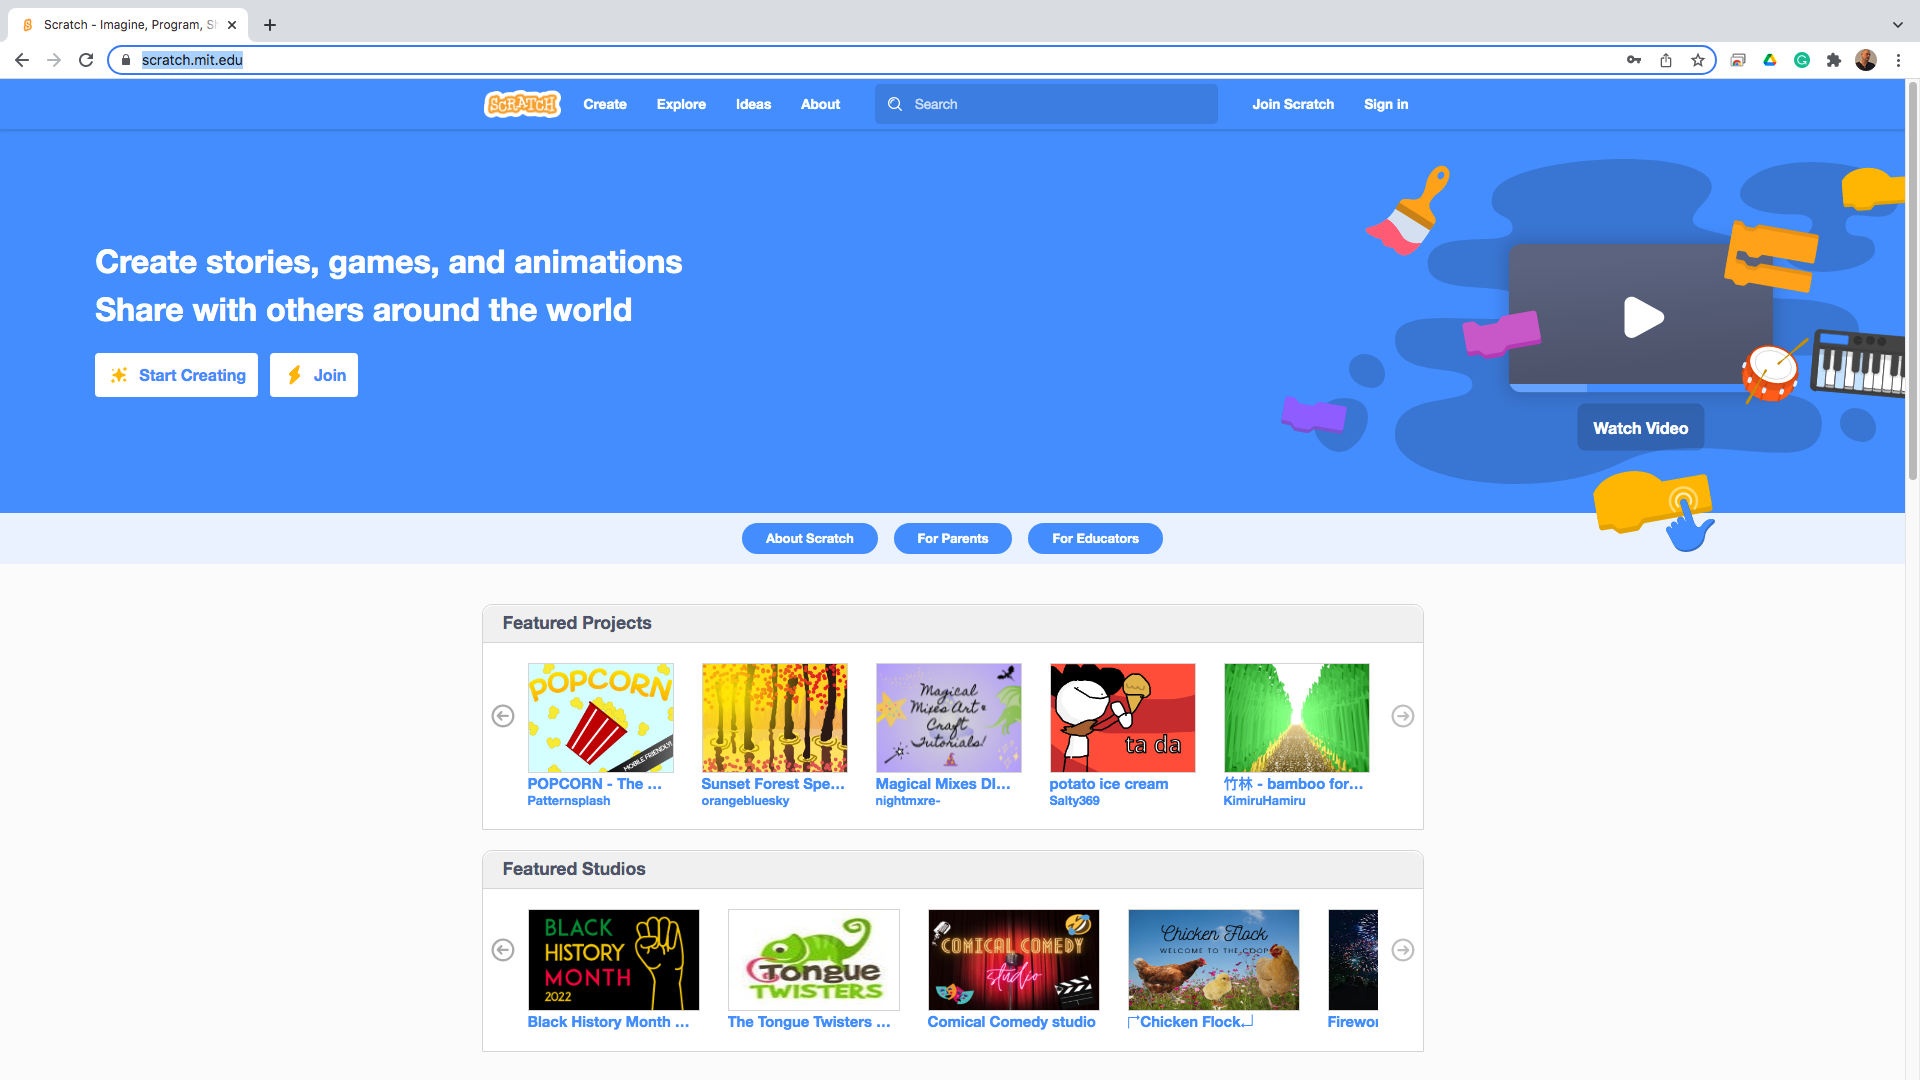
\includegraphics[width=1.0\linewidth,height=0.5\linewidth]{fig0001.png}
  \caption{Начална уеб страница на Sratch}
\label{fig0001}
\end{figure}

Програмната среда на Sratch е организирана на принципа на облачните услуги. Поради тази причина, всеки желаещ да използва услугата трябва да си направи регистрация (Фиг. \ref{fig0002}). Регистрацията се състои от потребителско име и парола.

\begin{figure}[H]
  \centering
  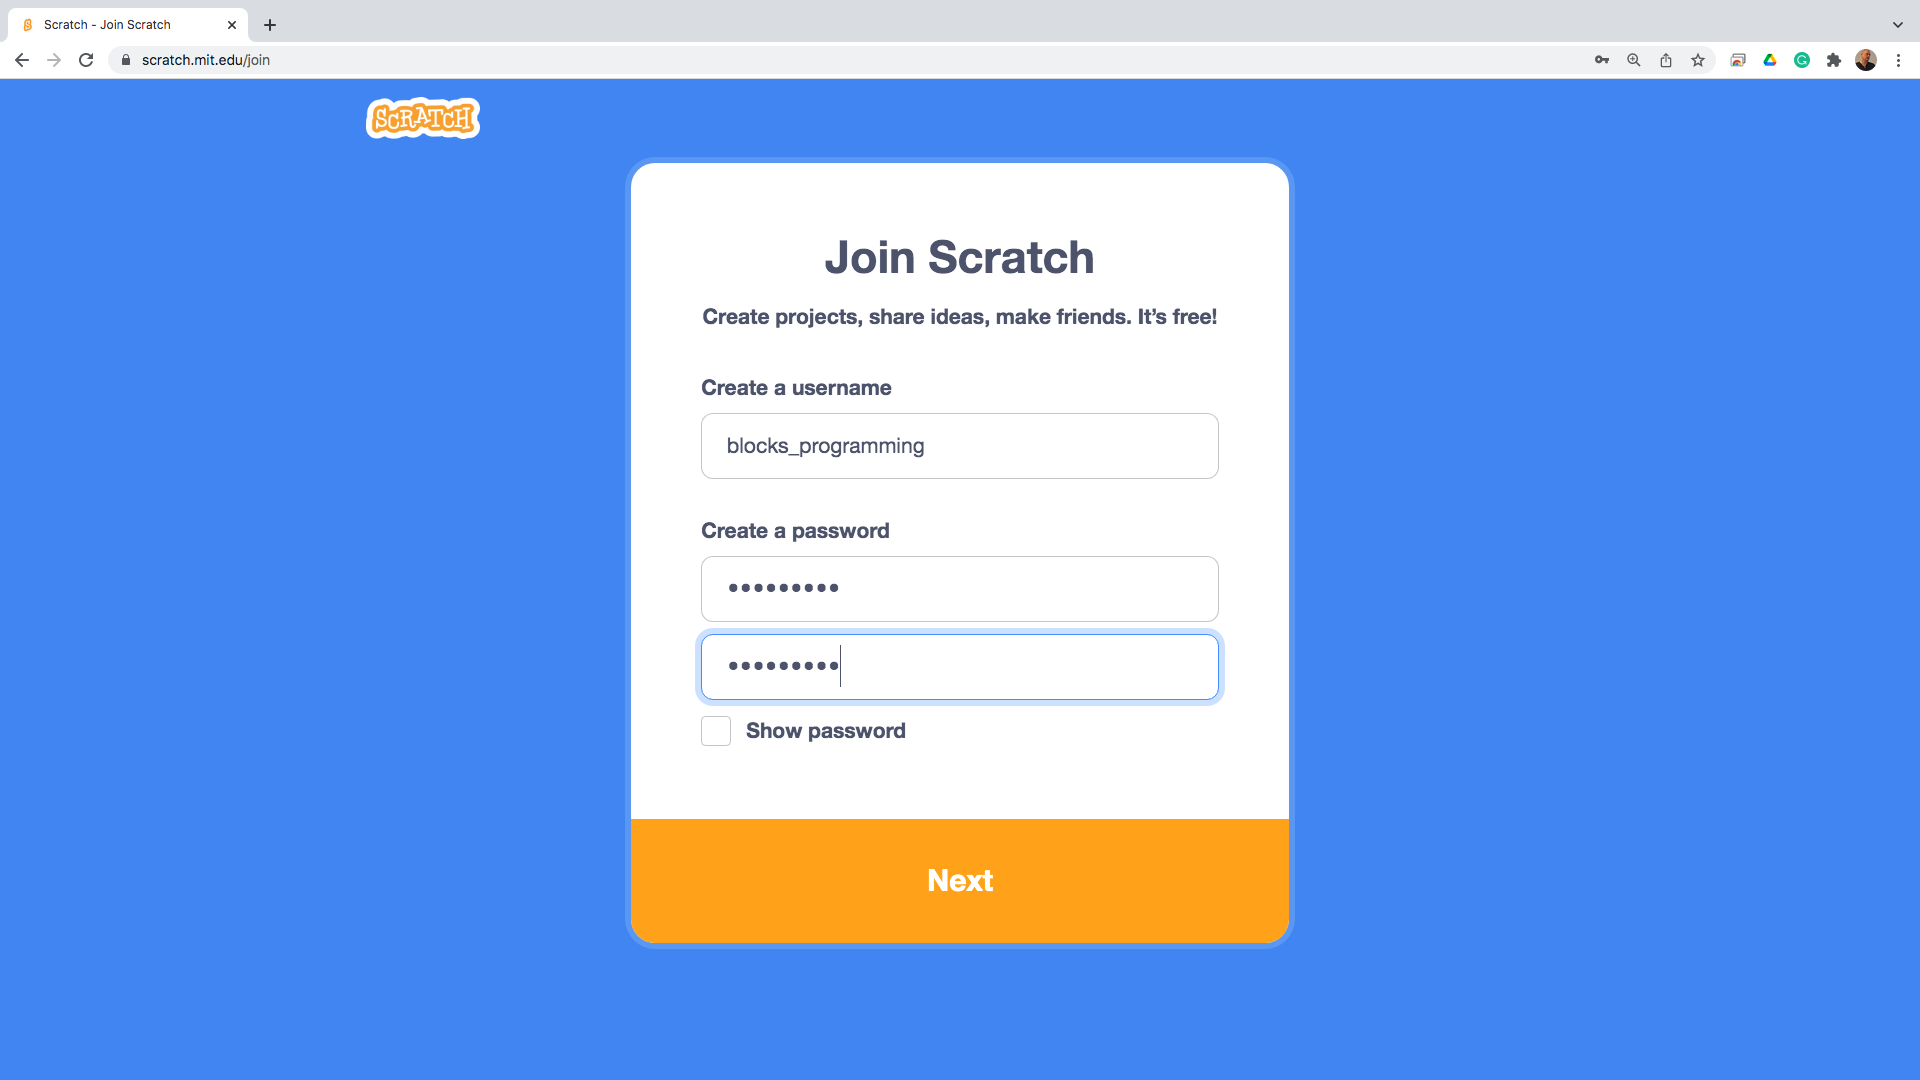
\includegraphics[width=1.0\linewidth,height=0.5\linewidth]{fig0002.png}
  \caption{Регистрация на потребител в Sratch}
\label{fig0002}
\end{figure}

След избора на потребителско име и парола следва определяне на географския регион в който се намира потребителят (Фиг. \ref{fig0003}).

\begin{figure}[H]
  \centering
  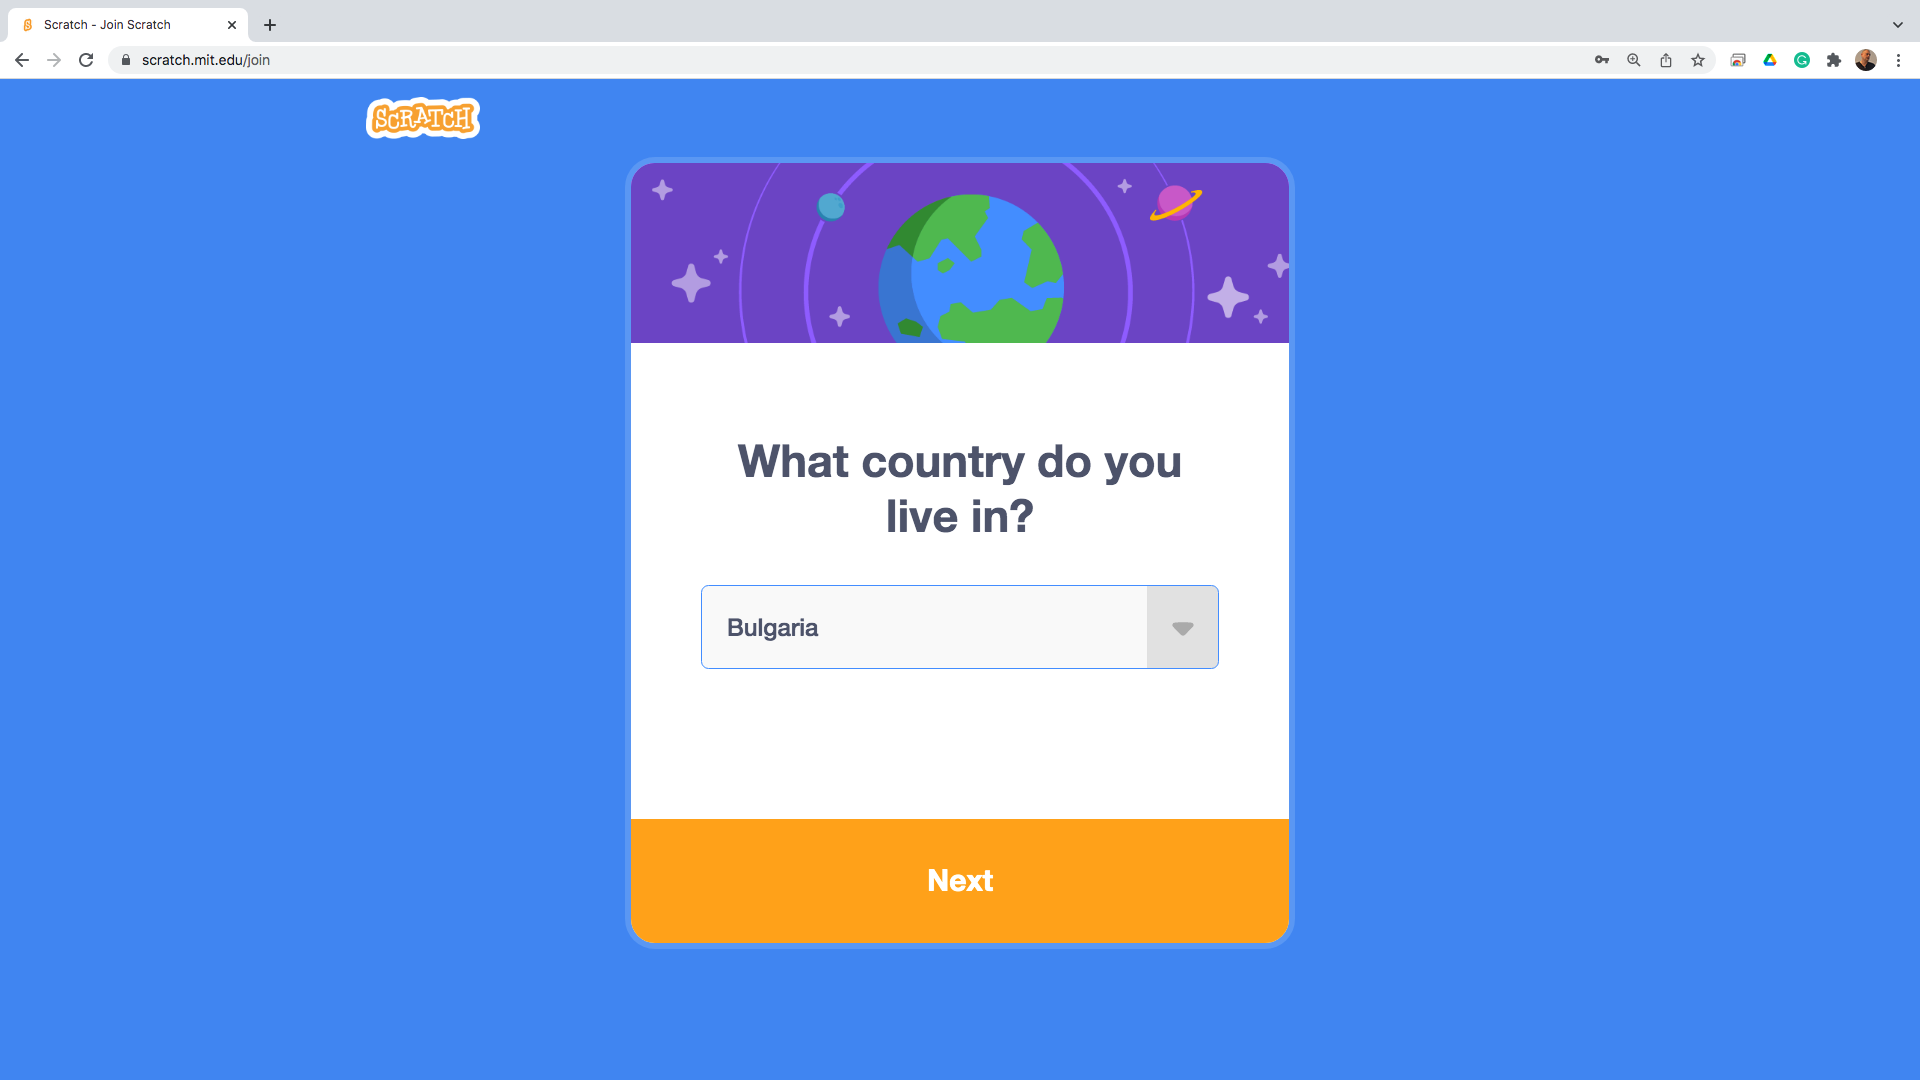
\includegraphics[width=1.0\linewidth,height=0.5\linewidth]{fig0003.png}
  \caption{Географско местоположение}
\label{fig0003}
\end{figure}

Платформата е насочена предимно към деца, изразяващи интерес към програмирането, но също така към родители и учители. Поради тази причина, системата събира информация за възрастта на потребителя (Фиг. \ref{fig0004}).

\begin{figure}[H]
  \centering
  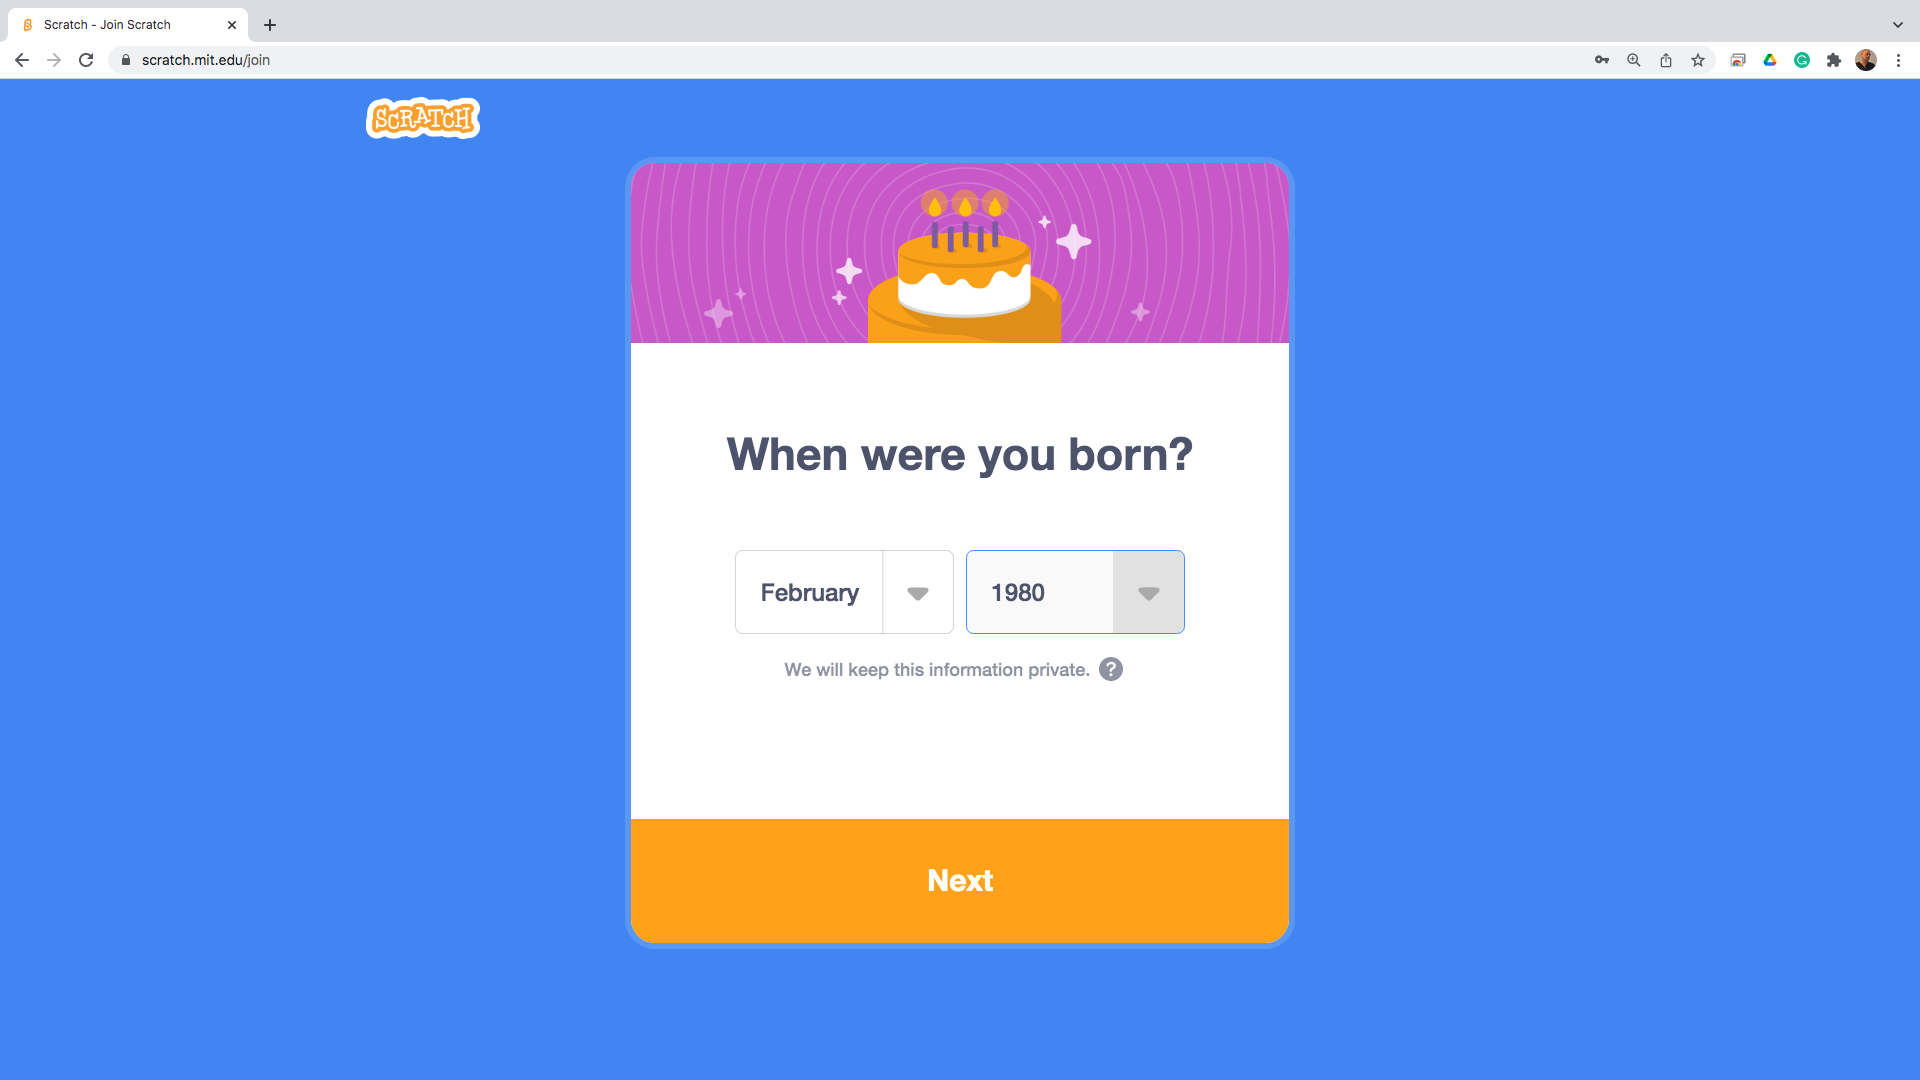
\includegraphics[width=1.0\linewidth,height=0.5\linewidth]{fig0004.png}
  \caption{Възраст на потребителя}
\label{fig0004}
\end{figure}

Освен класификация по възраст, системата събира информация и за класификация по полова принадлежност. Тази информация е незадължителна, основно за да не бъде дискриминираща (Фиг. \ref{fig0005}).

\begin{figure}[H]
  \centering
  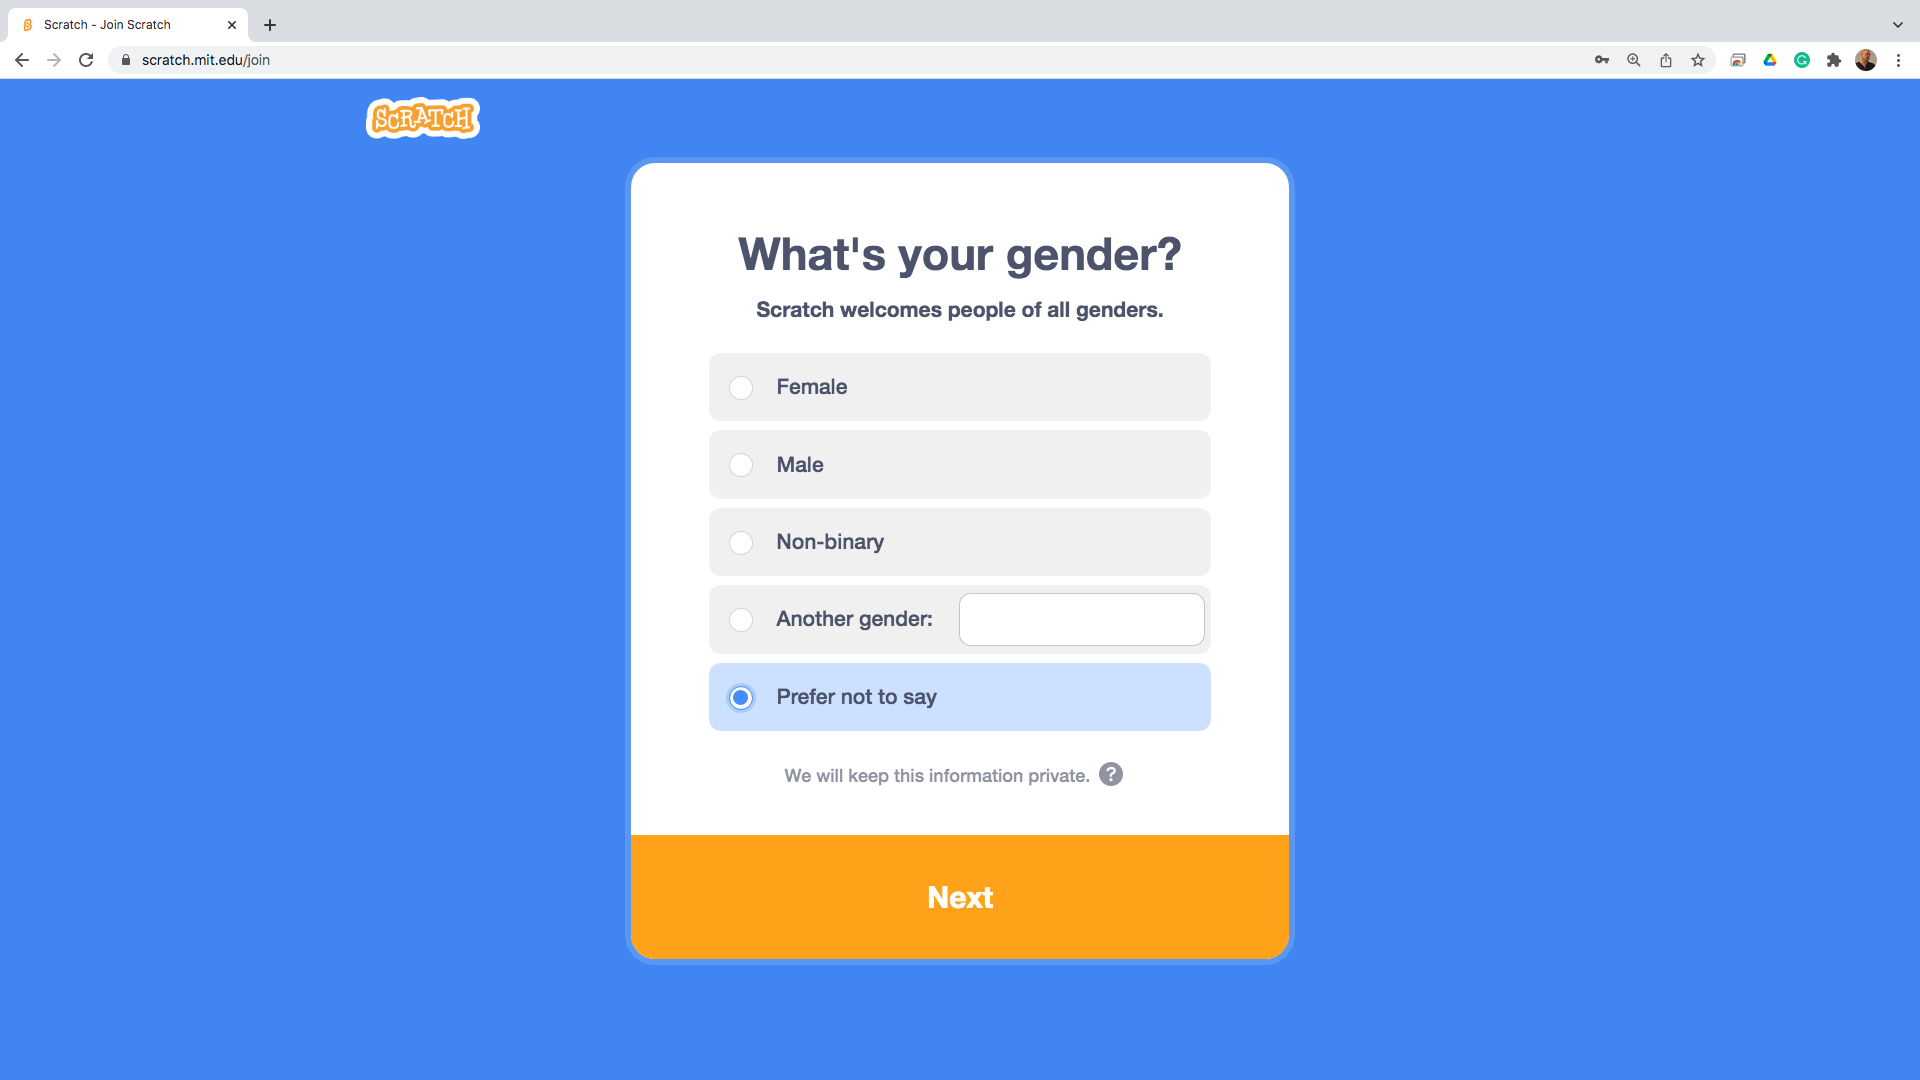
\includegraphics[width=1.0\linewidth,height=0.5\linewidth]{fig0005.png}
  \caption{Пол на потребителя}
\label{fig0005}
\end{figure}

Потребителският профил, освен с потребителско име и парола, трябва да бъде аоцииран и с адрес на електронна пощенска кутия (Фиг. \ref{fig0006}).

\begin{figure}[H]
  \centering
  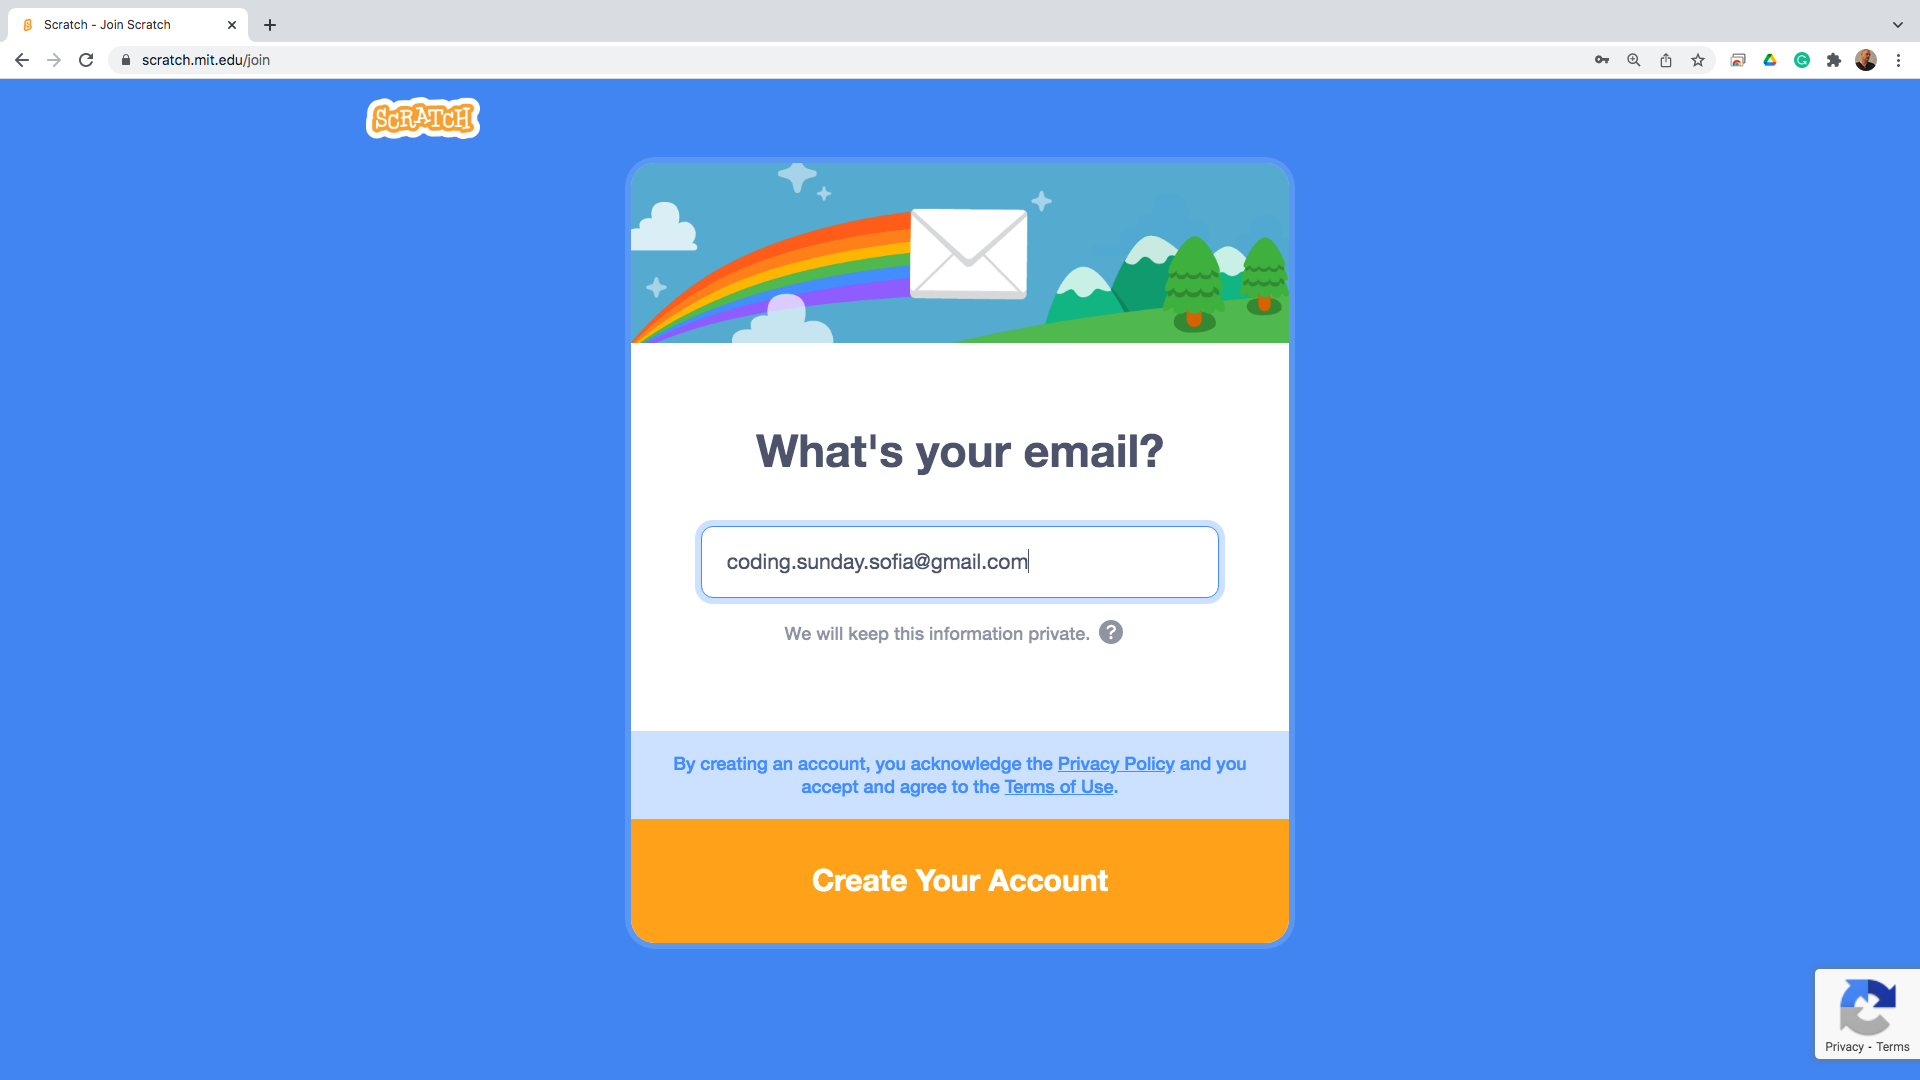
\includegraphics[width=1.0\linewidth,height=0.5\linewidth]{fig0006.png}
  \caption{Адрес на електронна поща на потребителя}
\label{fig0006}
\end{figure}

Процесът по регистрация на потребител в системата е почти завършен (Фиг. \ref{fig0007}). Остава само стъпката за потвърждаване на избрания адрес за електронна поща.

\begin{figure}[H]
  \centering
  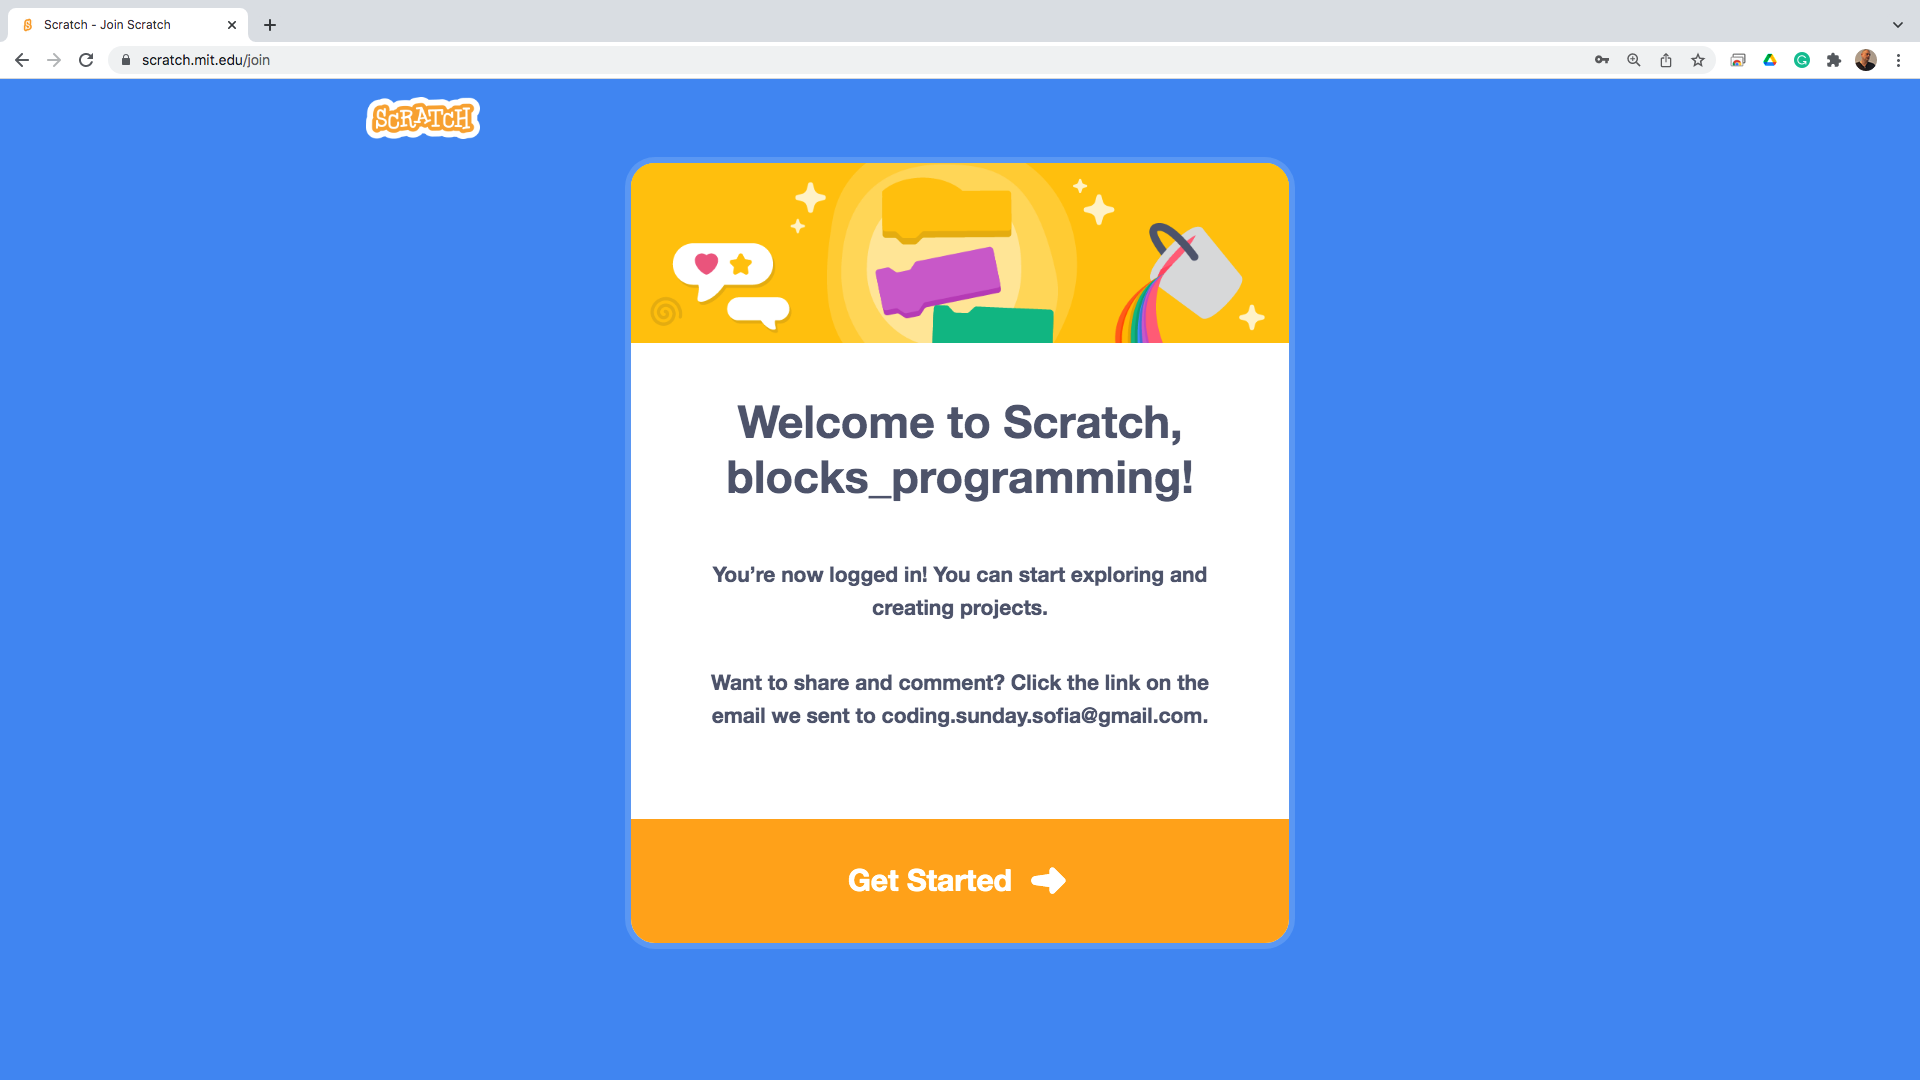
\includegraphics[width=1.0\linewidth,height=0.5\linewidth]{fig0007.png}
  \caption{Приключване на процеса за въвеждане на информация за потребителя}
\label{fig0007}
\end{figure}

Електронното писмо, за потвърждаване на потребителската регистрация, съдържа електронна препратка до уеб сайта на Sratch (Фиг. \ref{fig0008}). Тази препратка трябва да бъде последвана за да се завърши процесът по регистрация на нов потребител. 

\begin{figure}[H]
  \centering
  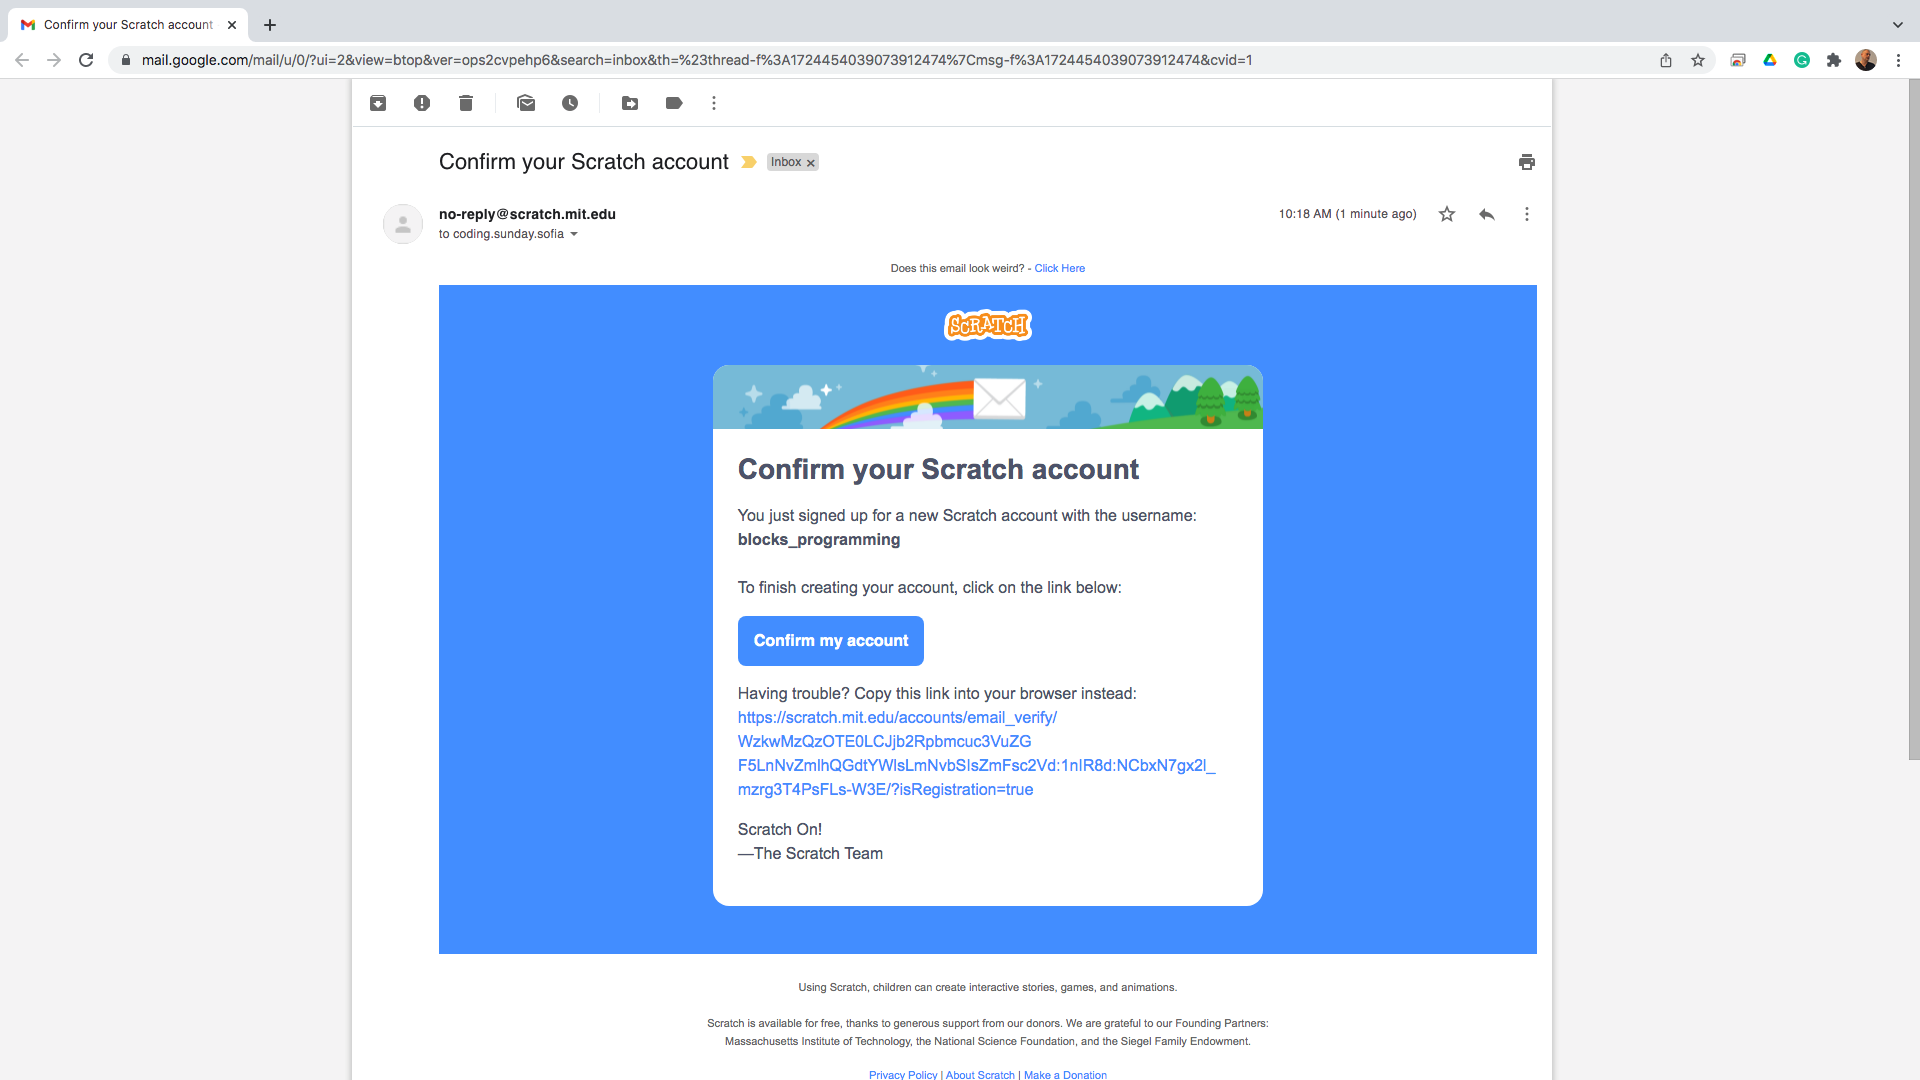
\includegraphics[width=1.0\linewidth,height=0.5\linewidth]{fig0008.png}
  \caption{Електронно съобщение за потвърждаване на електронния адрес}
\label{fig0008}
\end{figure}

Регистрацията на новия потребител приключва със зареждането на начален работен екран (Фиг. \ref{fig0009}). Горе, в дясно се вижда изписано потребителското име, избрано на първата стъпка от процеса по регистрацията.

\begin{figure}[H]
  \centering
  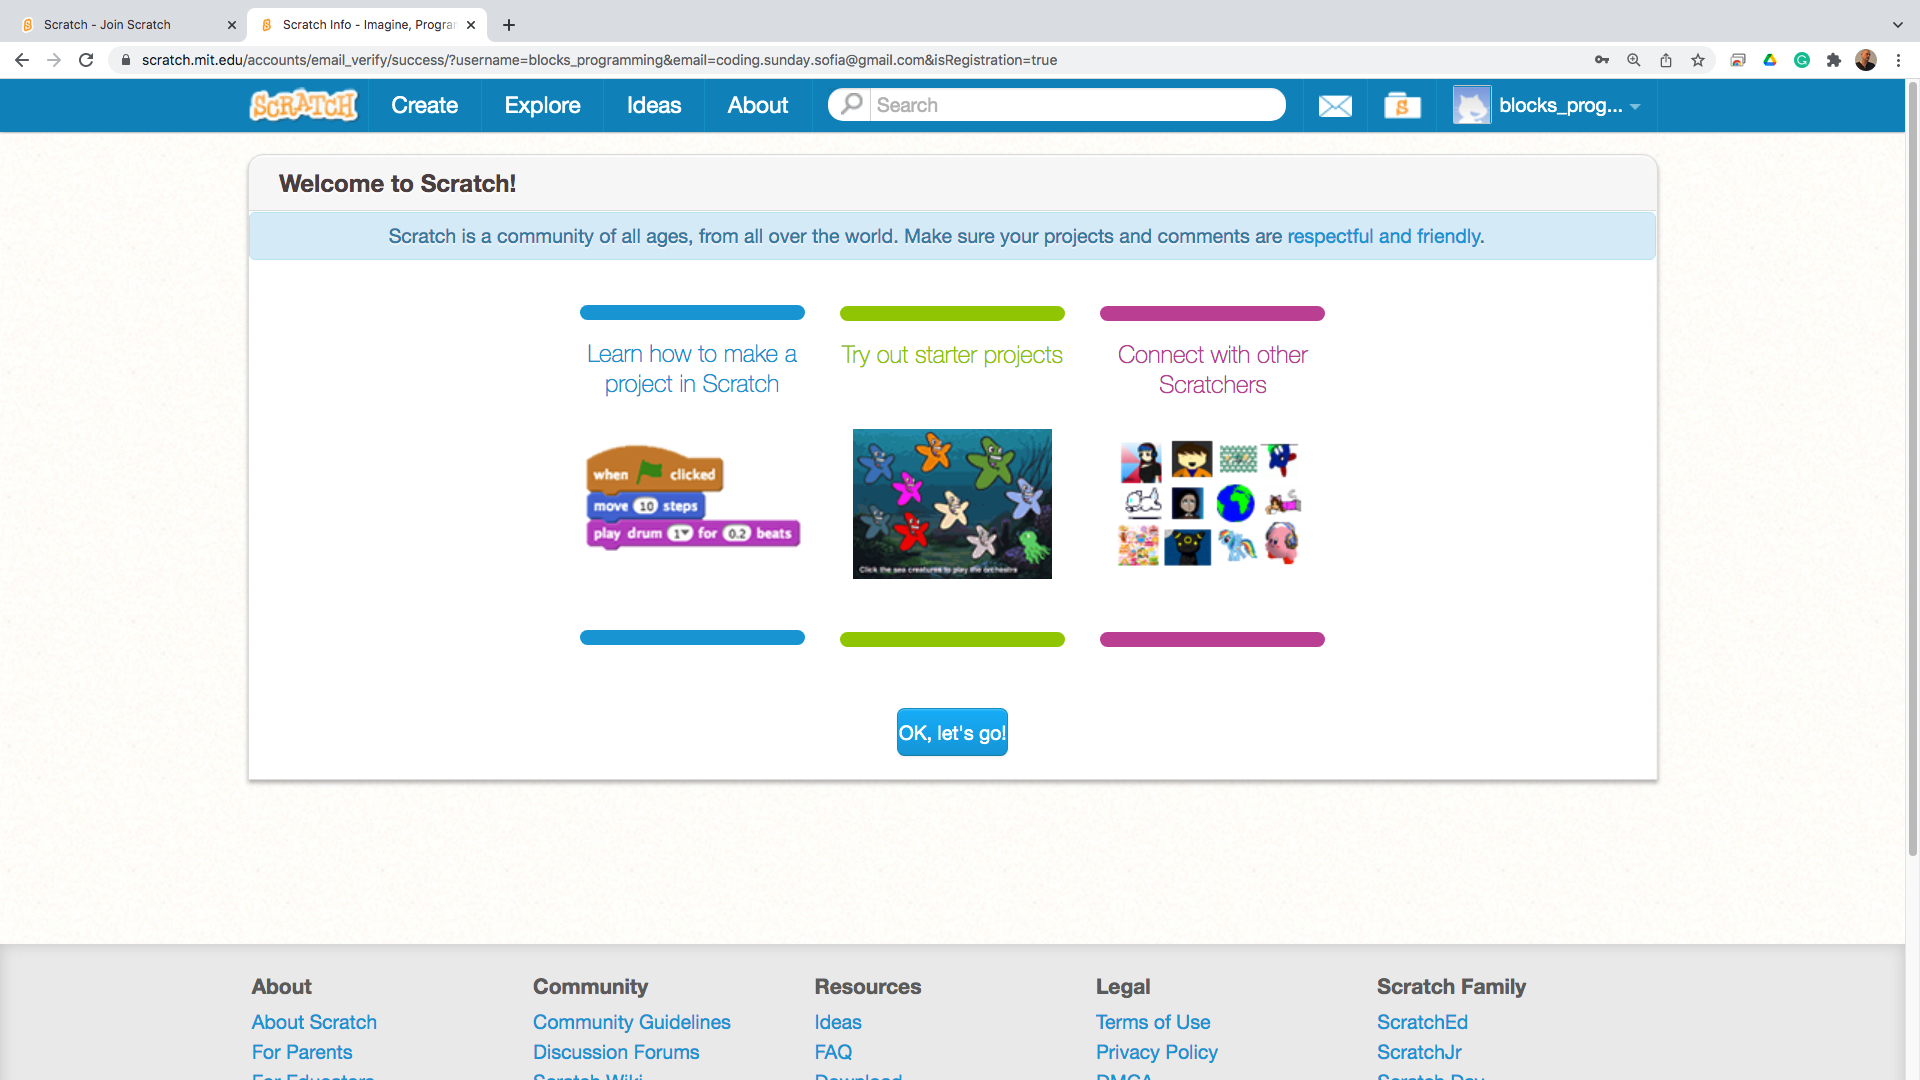
\includegraphics[width=1.0\linewidth,height=0.5\linewidth]{fig0009.png}
  \caption{Начален работен екран}
\label{fig0009}
\end{figure}

Успешната регистрация може да се потвърди и чрез създаването на много малък проект, който да демонстрира функционирането на развойната среда. За тази цел се избира опцията „Create“ от менюто (Фиг. \ref{fig0010}).

\begin{figure}[H]
  \centering
  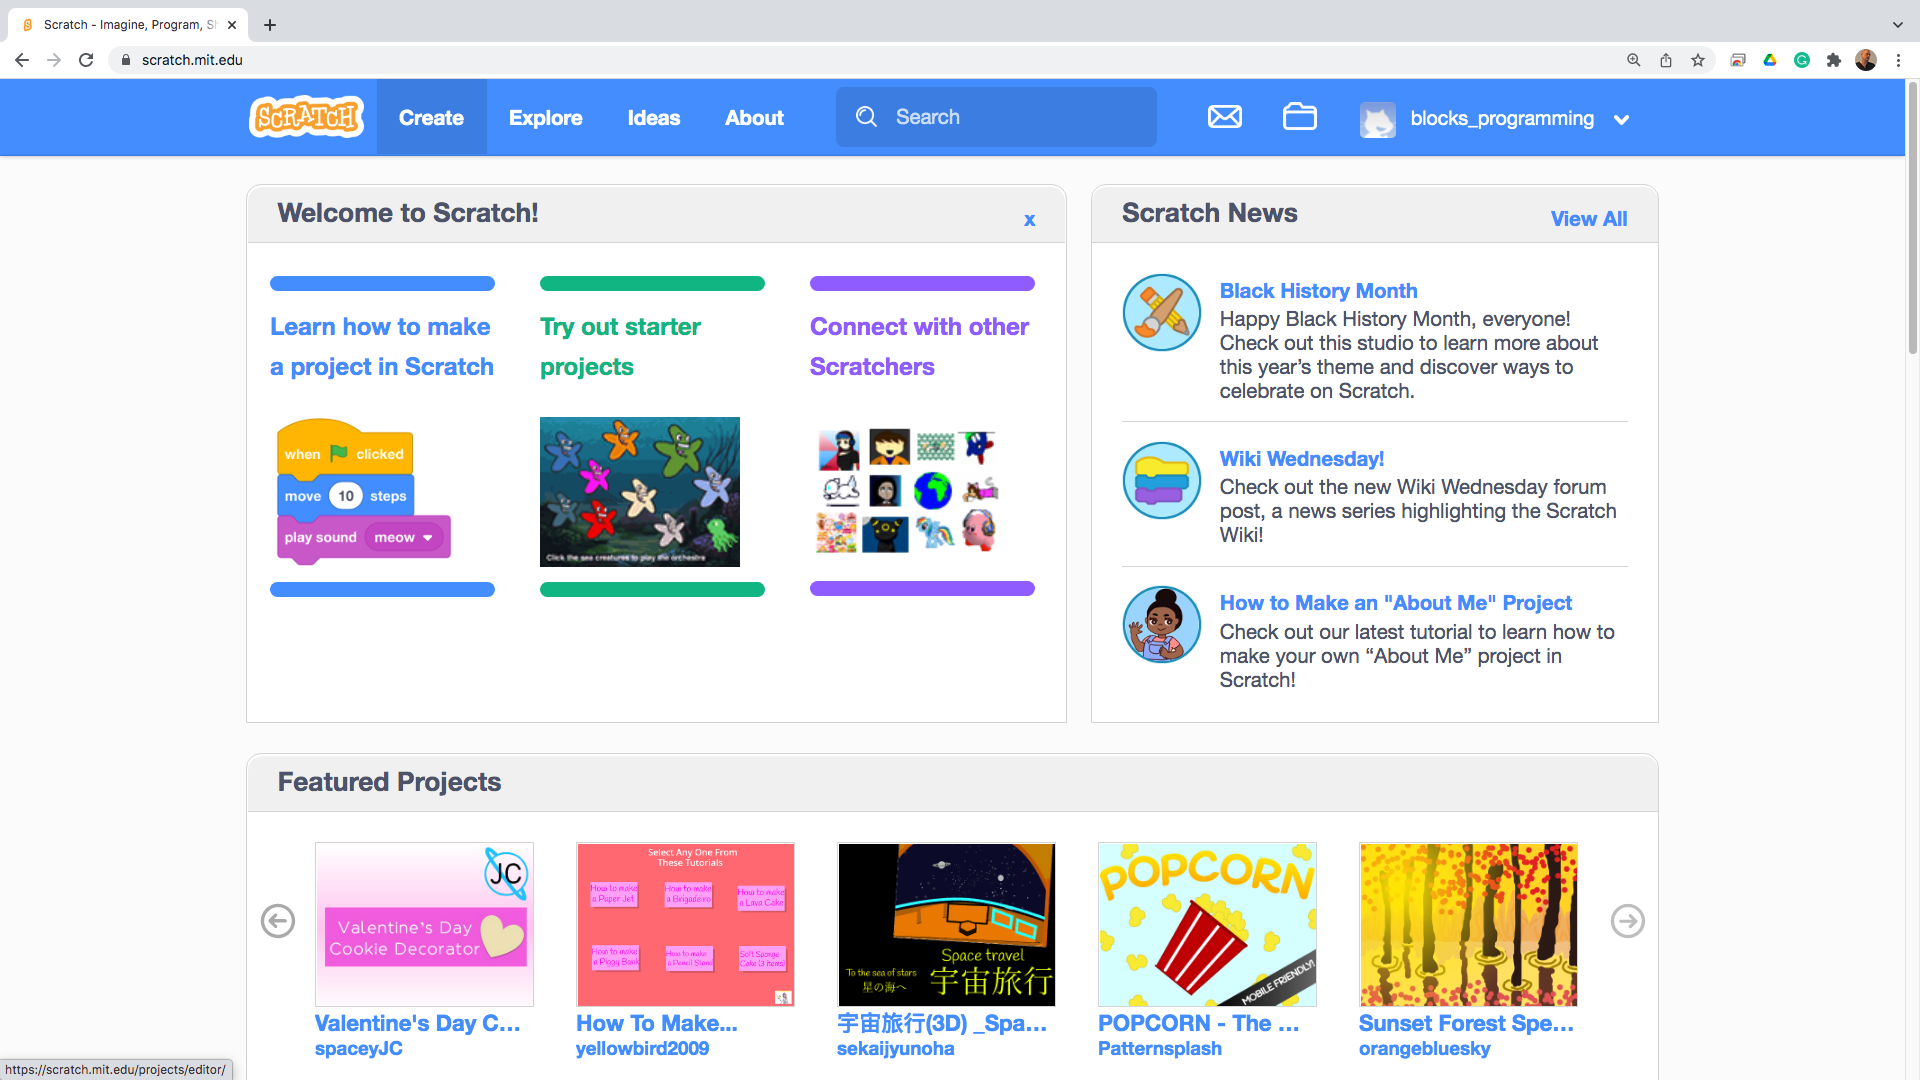
\includegraphics[width=1.0\linewidth,height=0.5\linewidth]{fig0010.png}
  \caption{Избор на опция от менюто за нов проект}
\label{fig0010}
\end{figure}

Създаването на нов проект преминава през серия стъпки, свързани със заделянето на първоначално нужните ресурси (Фиг. \ref{fig0011}).

\begin{figure}[H]
  \centering
  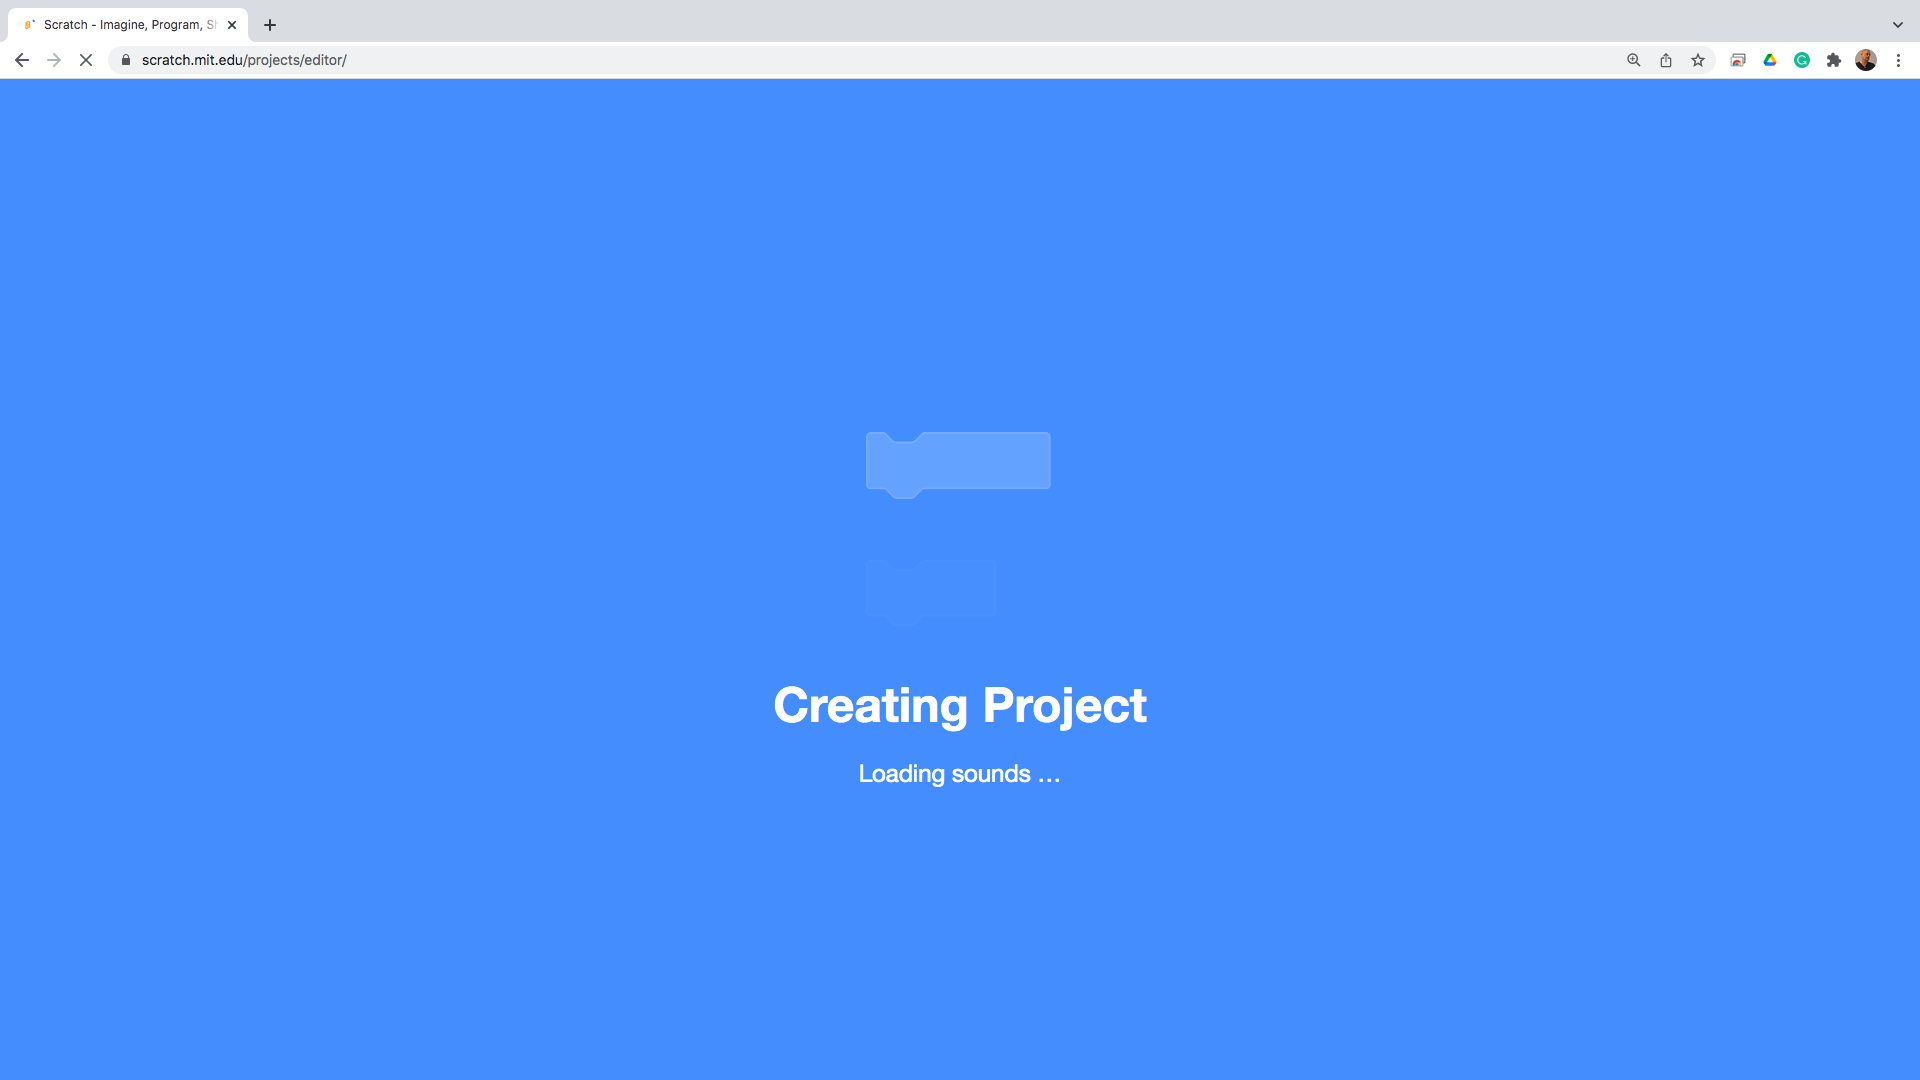
\includegraphics[width=1.0\linewidth,height=0.5\linewidth]{fig0011.png}
  \caption{Зареждане на ресурсите}
\label{fig0011}
\end{figure}

След зареждането на новия проект се визуализира работното пространство (Фиг. \ref{fig0012}). Най- в ляво е списъкът с възможни програмни инструкции, под формата на парченца от пъзел. В централната част е работното пространство, където инструкциите се подреждат. А най- в дясно е активната сцена, където се визуализират действията, заложени в серията от инструкции. 

\begin{figure}[H]
  \centering
  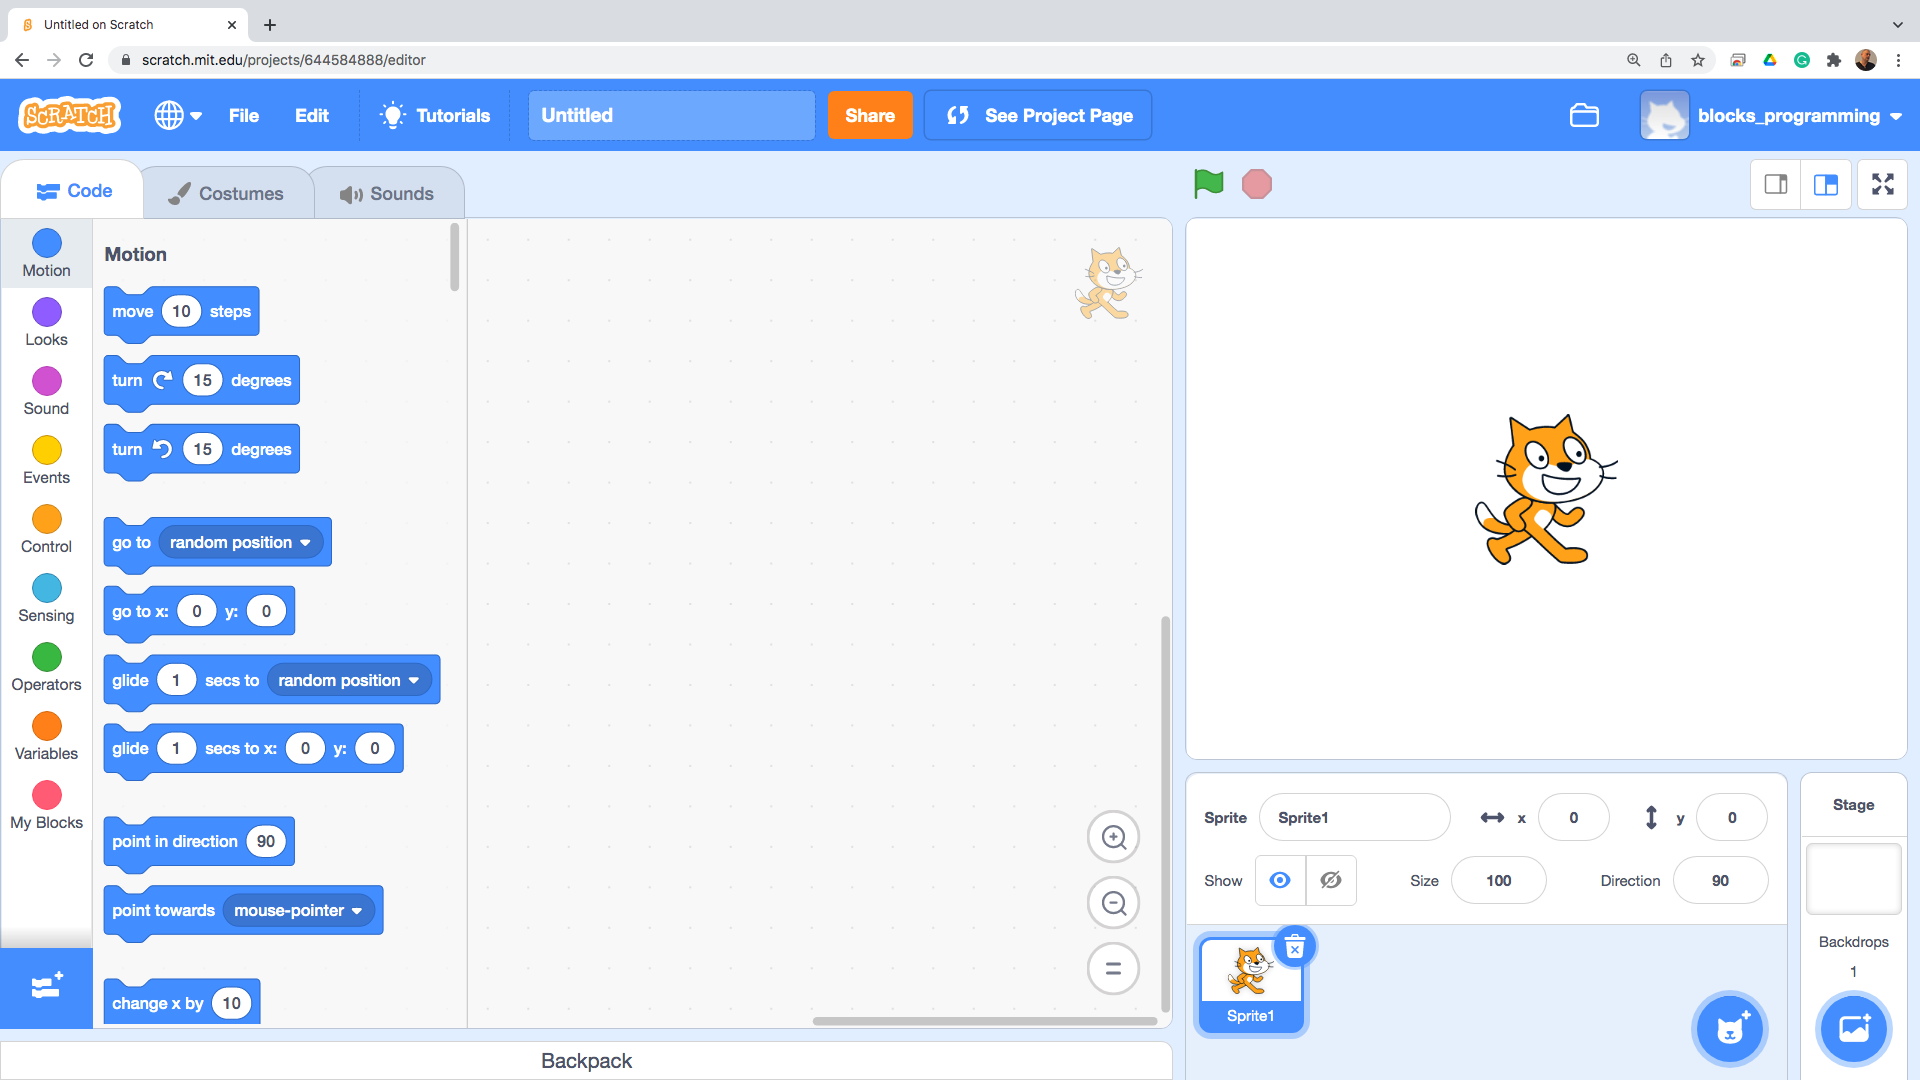
\includegraphics[width=1.0\linewidth,height=0.5\linewidth]{fig0012.png}
  \caption{Организация на работното пространство}
\label{fig0012}
\end{figure}

Всяка компютърна програма има своя начална точка и своя крайна точка. В Scratch, за началото на програмата има специално отделен блок (програмна инструкция), която е показна на Фиг. \ref{fig0013}. Изпълнението на програмите, написани в Scratch, започва с натискането на зеления флаг. Точно поради тази причина, блокчето за старт на програмата е свързано със събитието за натискане на зеления флаг. 

\begin{figure}[H]
  \centering
  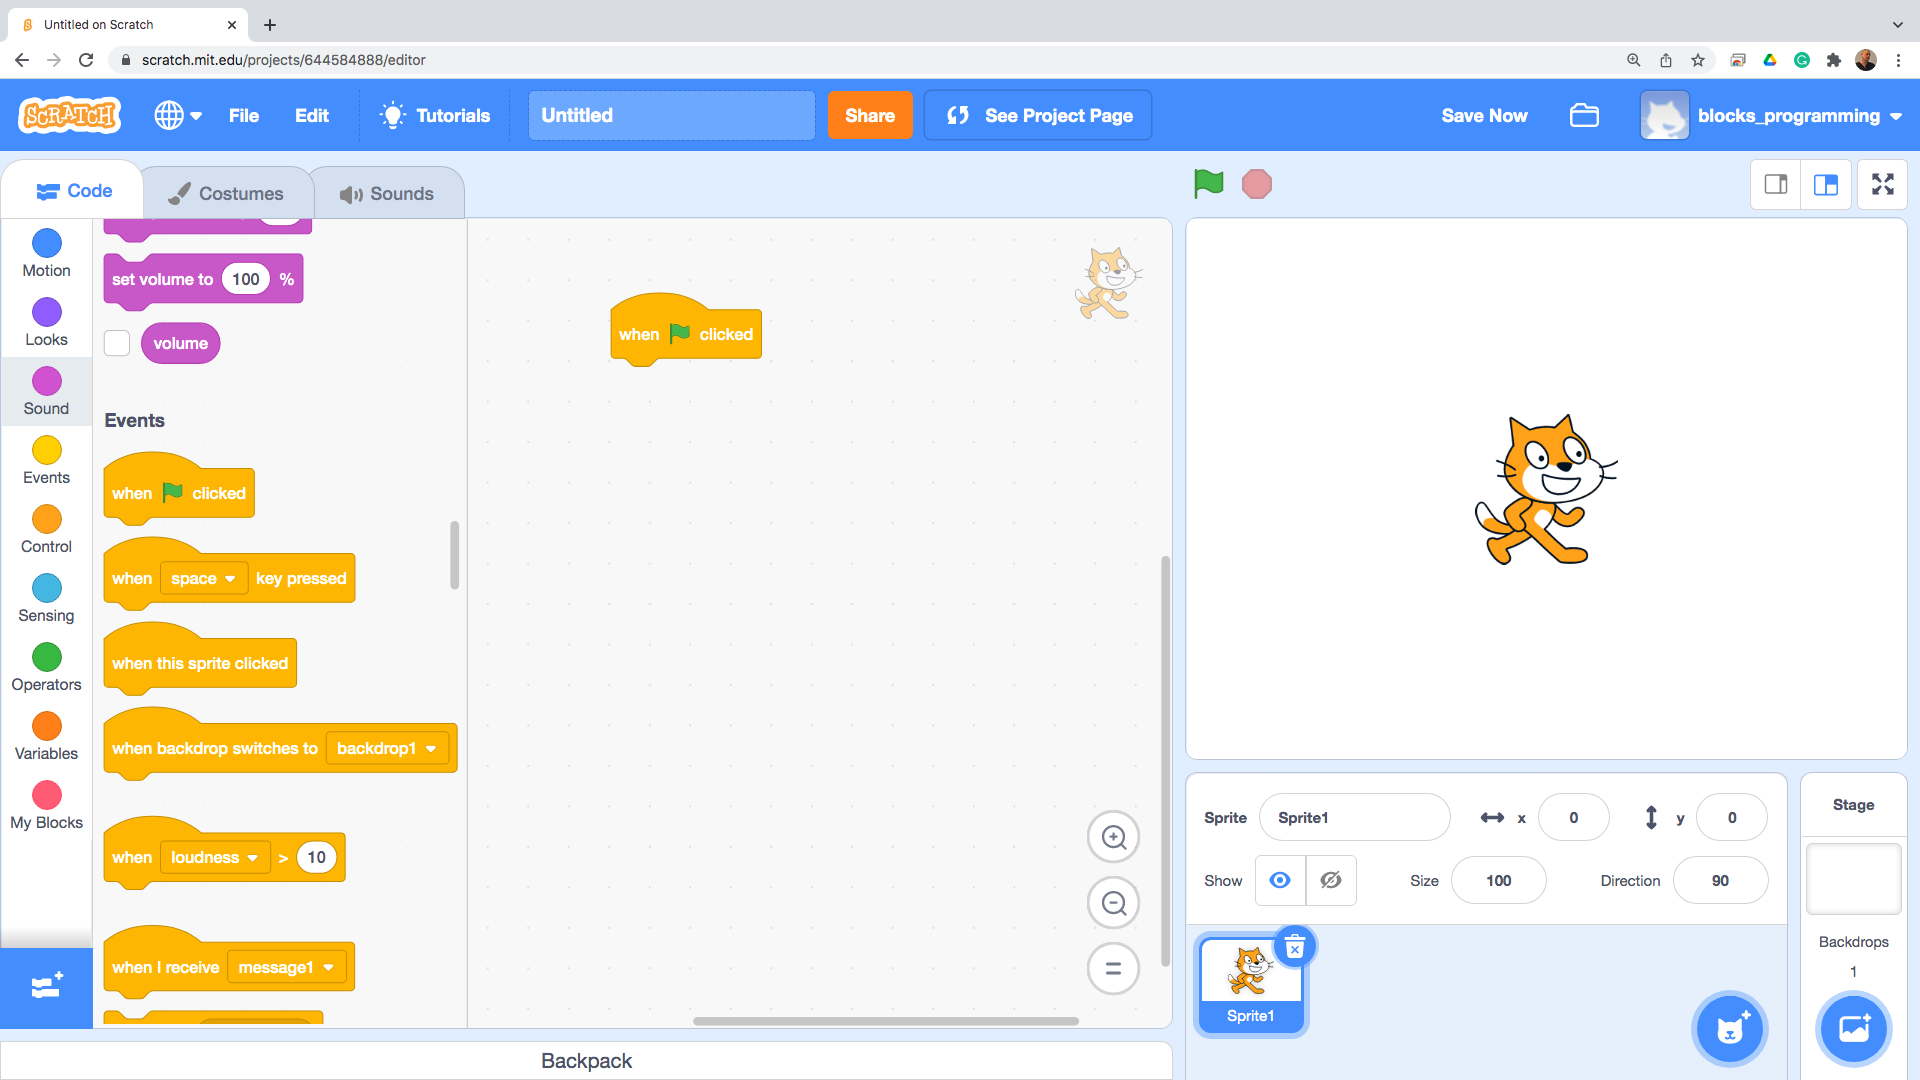
\includegraphics[width=1.0\linewidth,height=0.5\linewidth]{fig0013.png}
  \caption{Начало на програмата}
\label{fig0013}
\end{figure}

Една от най-интуитивните и същевременно лесно разбираеми инструкции е преместване с определен брой стъпки (Фиг. \ref{fig0014}). Главен актьор в началната сцена на Scratch е оранжевият котарак. Ако сцената не бъде променяна, то инструкциите за извършване на различни действия се насочват точно към този котарак. 

\begin{figure}[H]
  \centering
  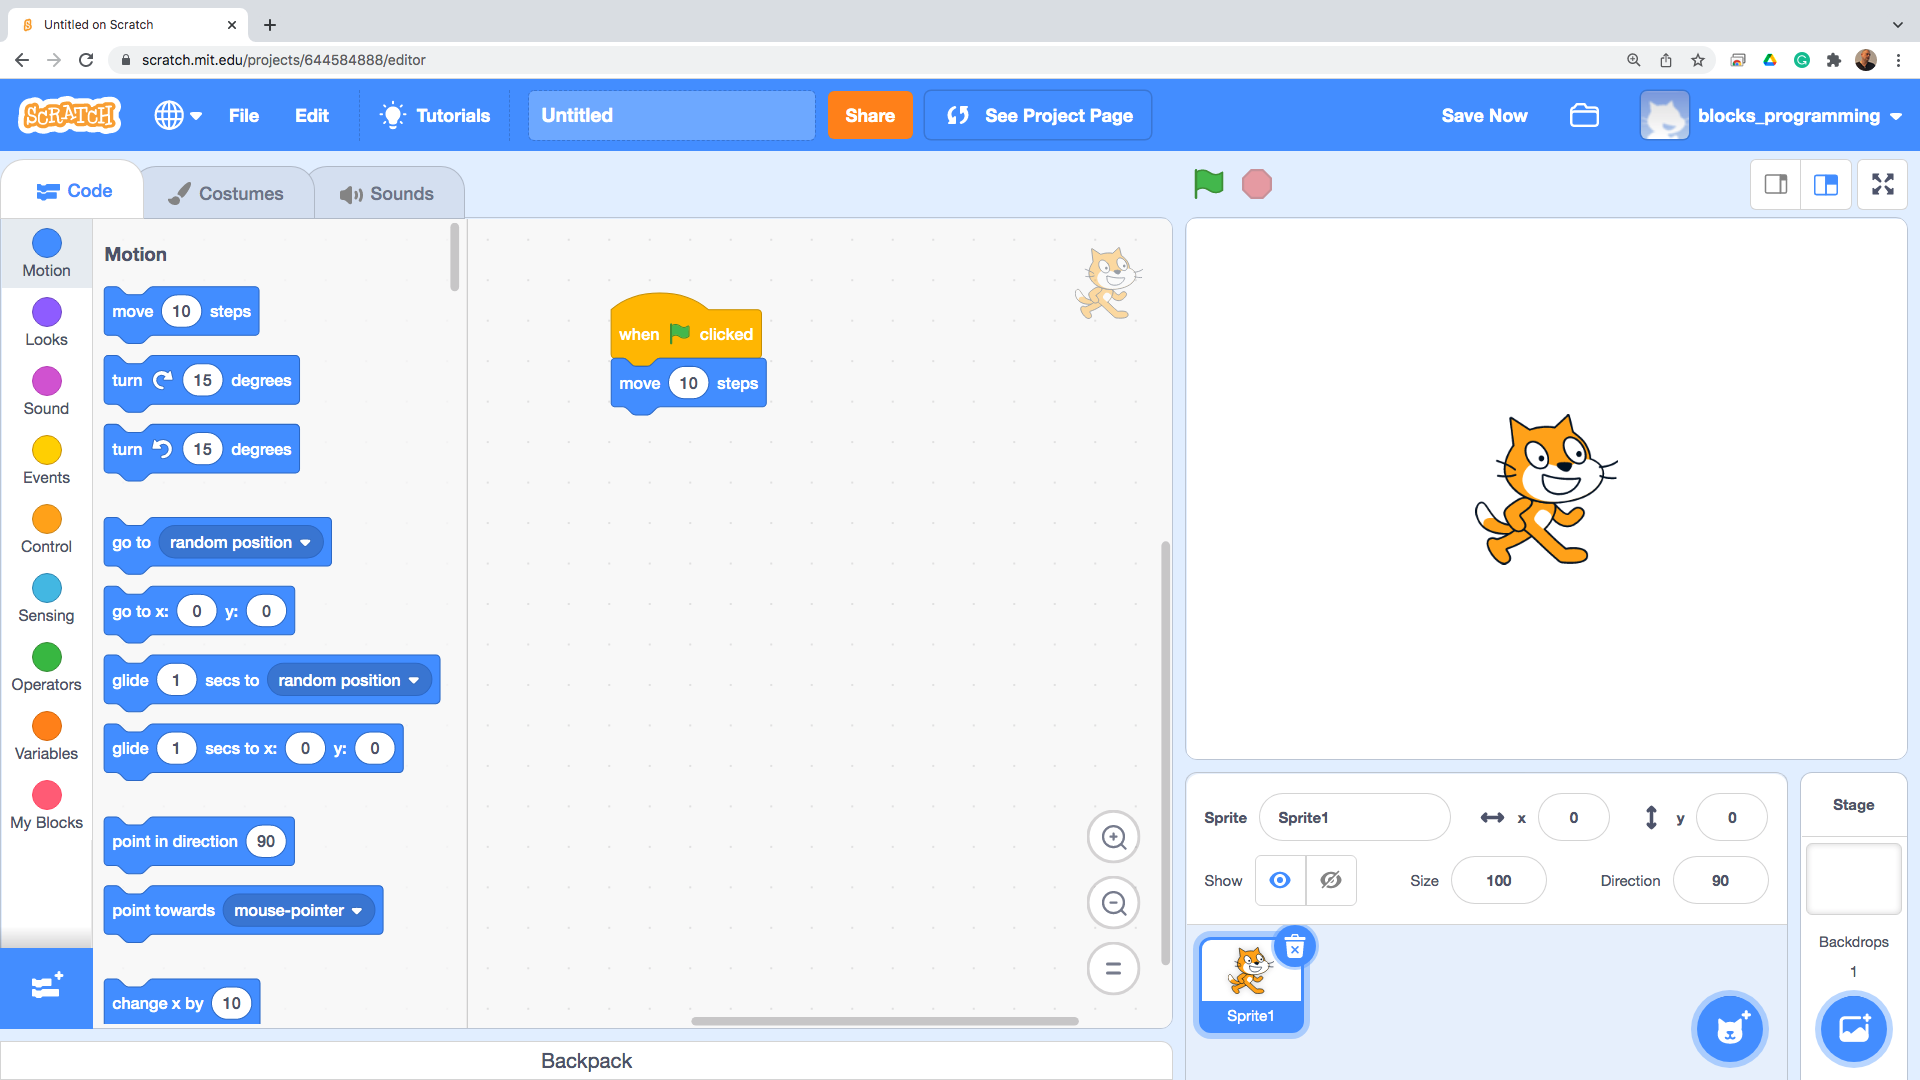
\includegraphics[width=1.0\linewidth,height=0.5\linewidth]{fig0014.png}
  \caption{Инструкция за придвижване на стъпки}
\label{fig0014}
\end{figure}

След преместването на котарака е от съществено значение да има една пауза на изчакване, така че визуално да се забележи преместването. За тази цел може да се приложи инструкция за изчакване, за определен брой секунди (Фиг. \ref{fig0015}).

\begin{figure}[H]
  \centering
  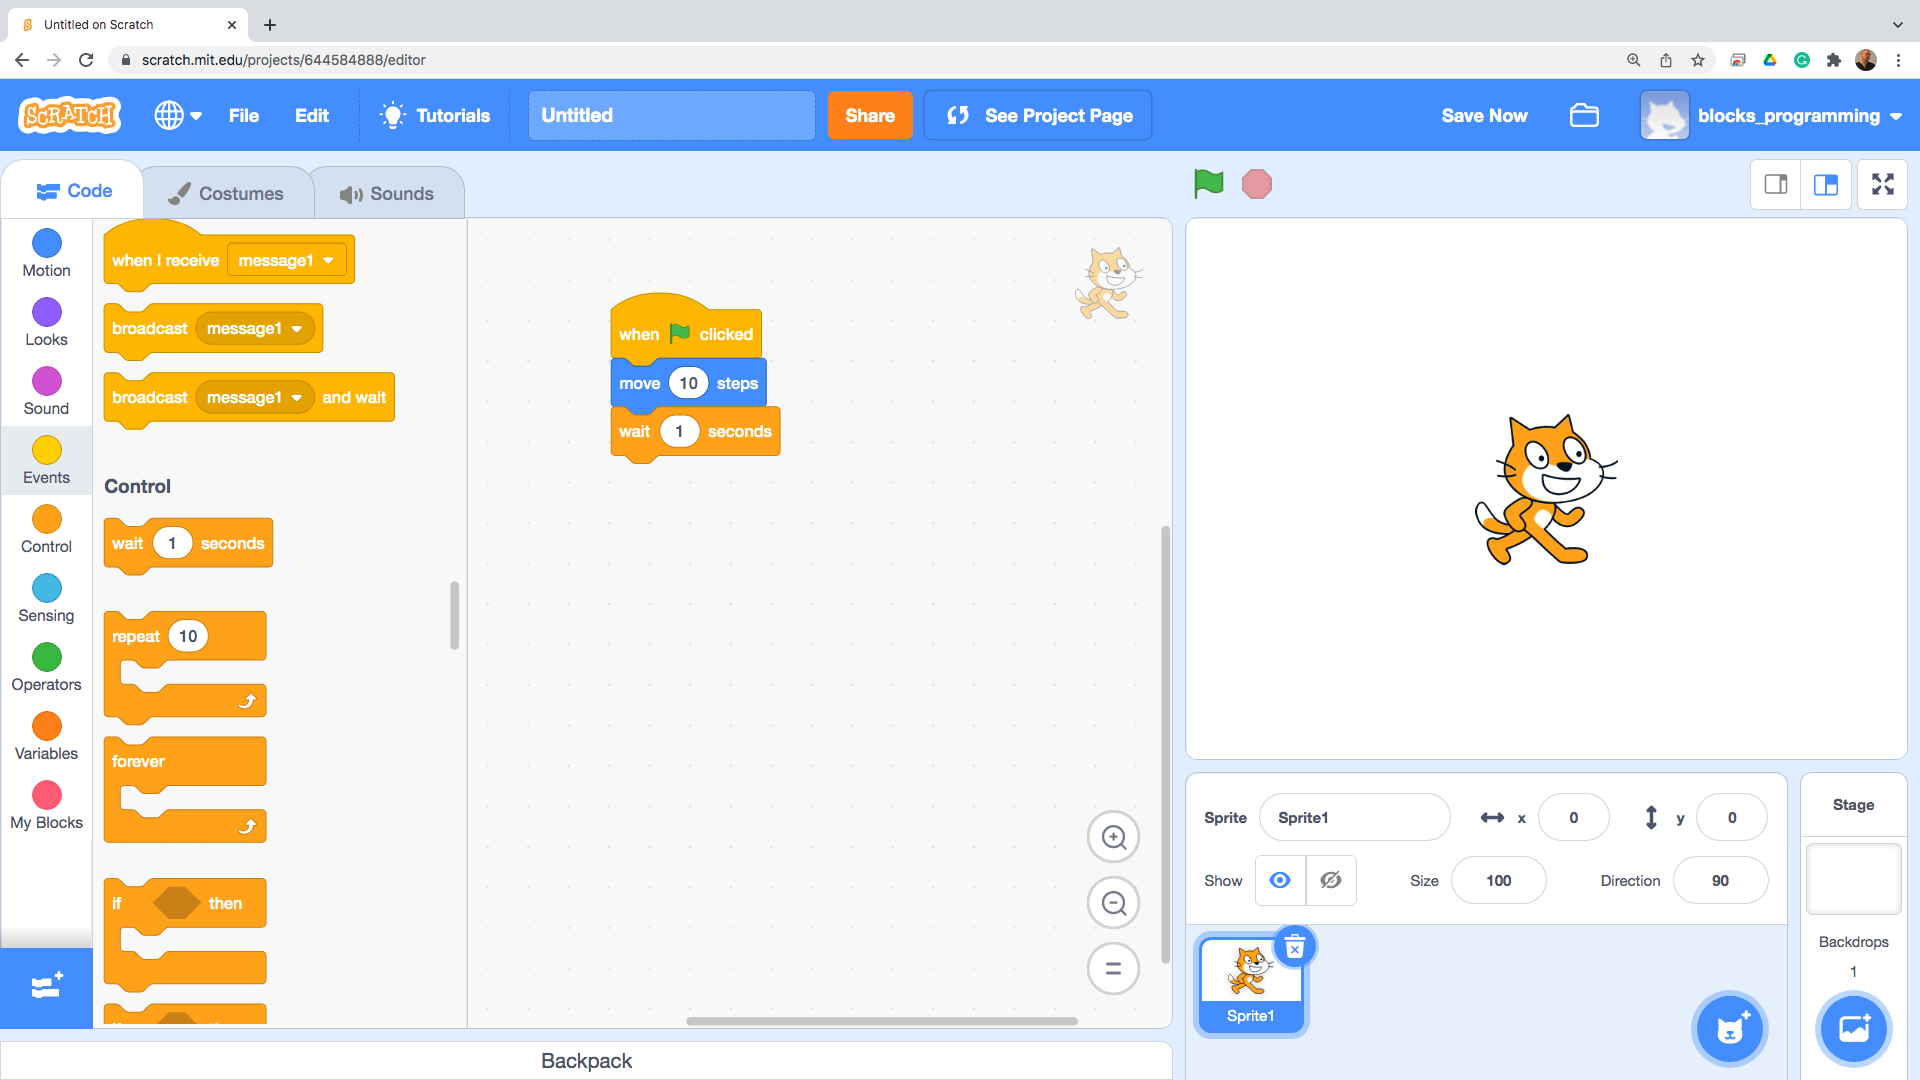
\includegraphics[width=1.0\linewidth,height=0.5\linewidth]{fig0015.png}
  \caption{Инструкция за изчакване}
\label{fig0015}
\end{figure}

След изчакването, котката може да се върне на първоначалната си позиция, като се изпълни инструкция за придвижване с отрицателен брой стъпки (Фиг. \ref{fig0016}).

\begin{figure}[H]
  \centering
  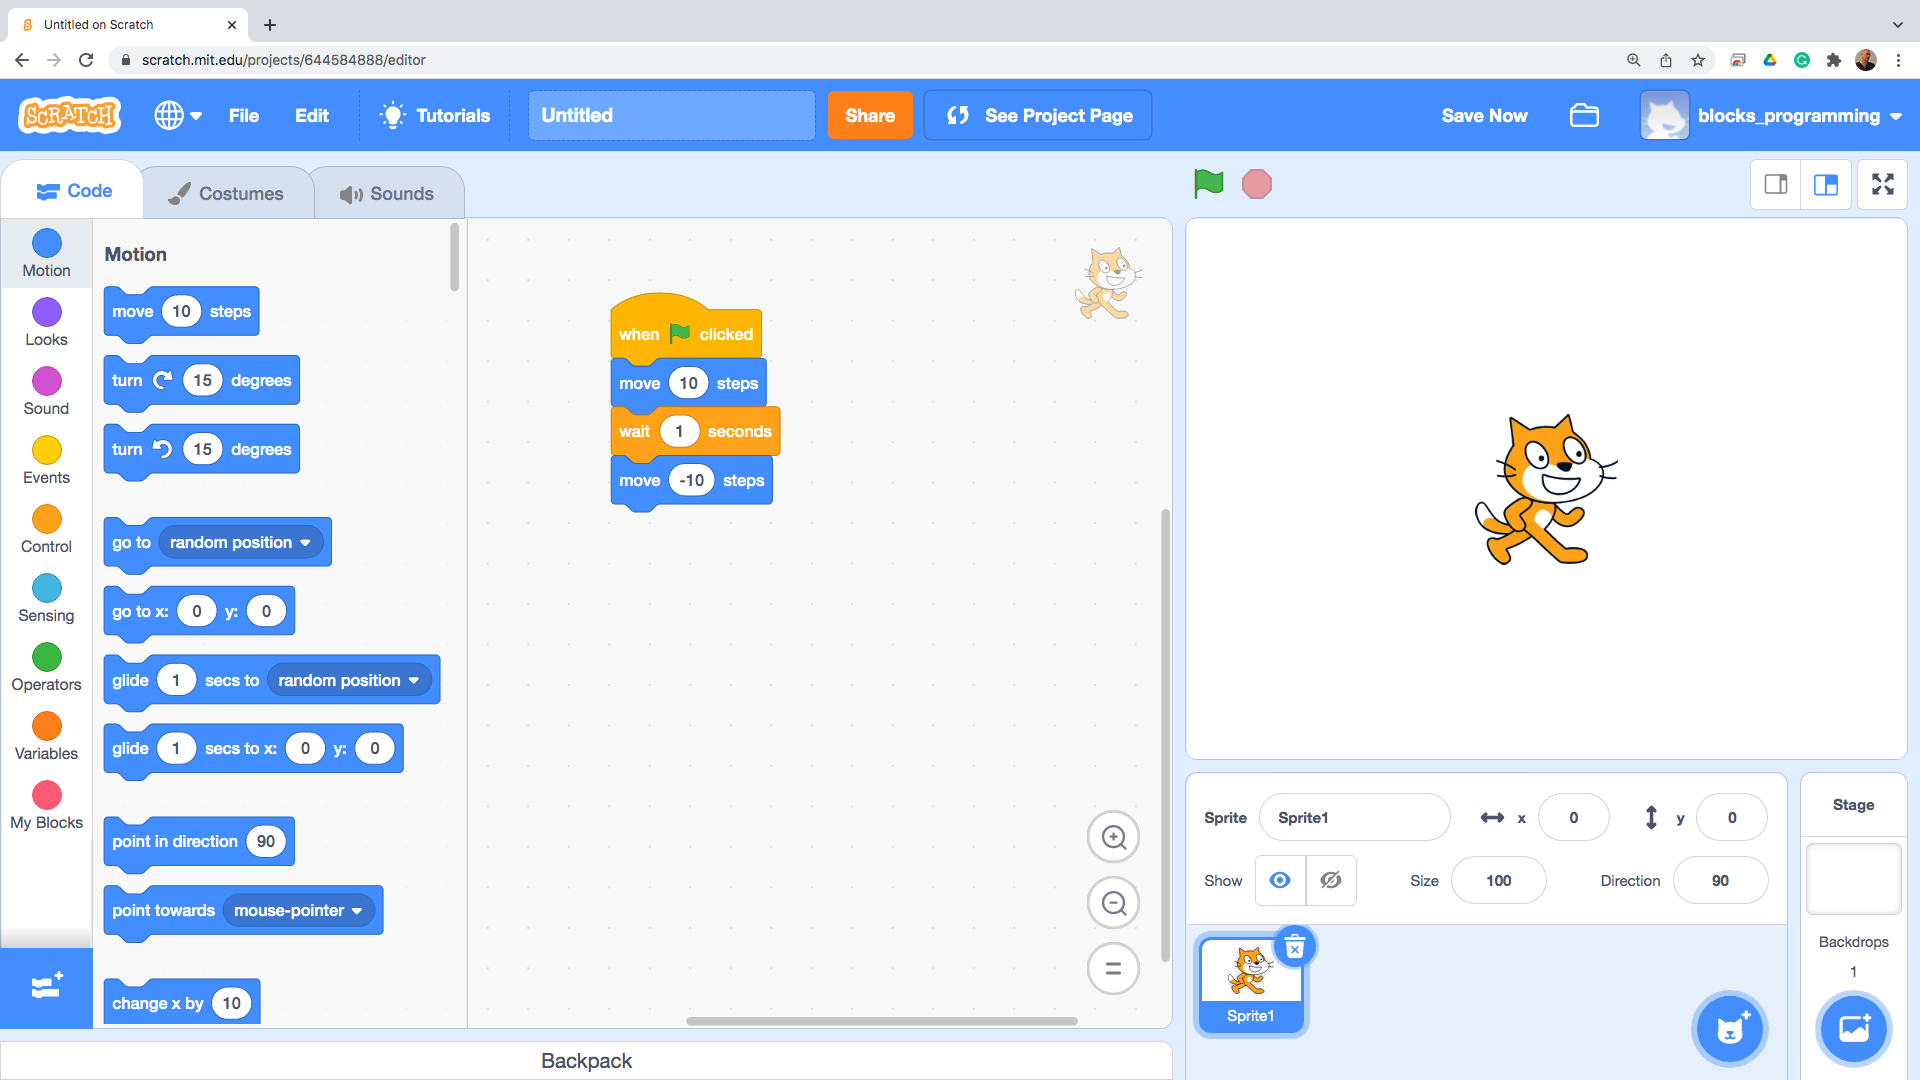
\includegraphics[width=1.0\linewidth,height=0.5\linewidth]{fig0016.png}
  \caption{Инструкция за преместване обратно}
\label{fig0016}
\end{figure}

След като всички предвидени инструкции са изпълнени е разумно да се сложи край на програмата, за което е предвидено отделно блокче в списъка с инструкции (Фиг. \ref{fig0017}).

\begin{figure}[H]
  \centering
  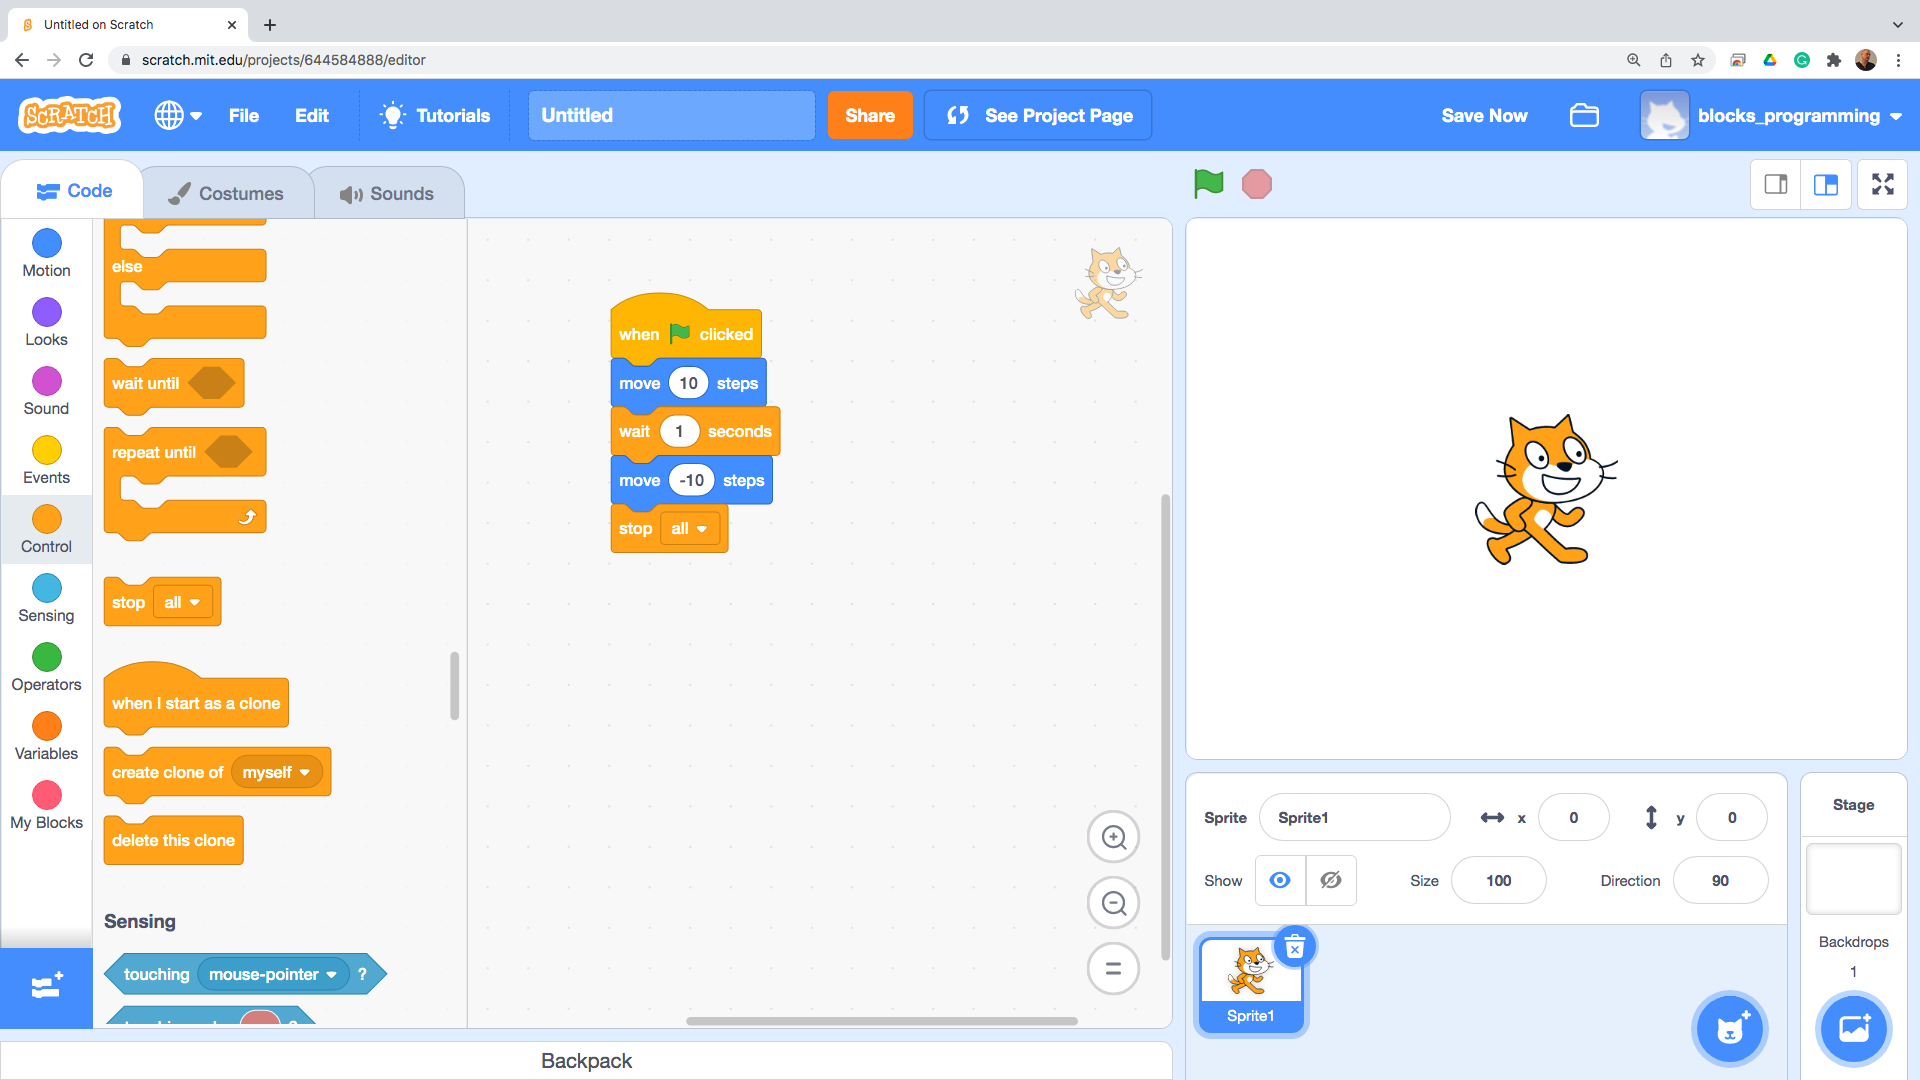
\includegraphics[width=1.0\linewidth,height=0.5\linewidth]{fig0017.png}
  \caption{Инструкция за край}
\label{fig0017}
\end{figure}

Така написаната програма се изпълнява, чрез натискане на зеления флаг (Фиг. \ref{fig0018}), а при нужда от аварийно спиране се натиска червеният кръг, от дясно на зеления флаг.

\begin{figure}[H]
  \centering
  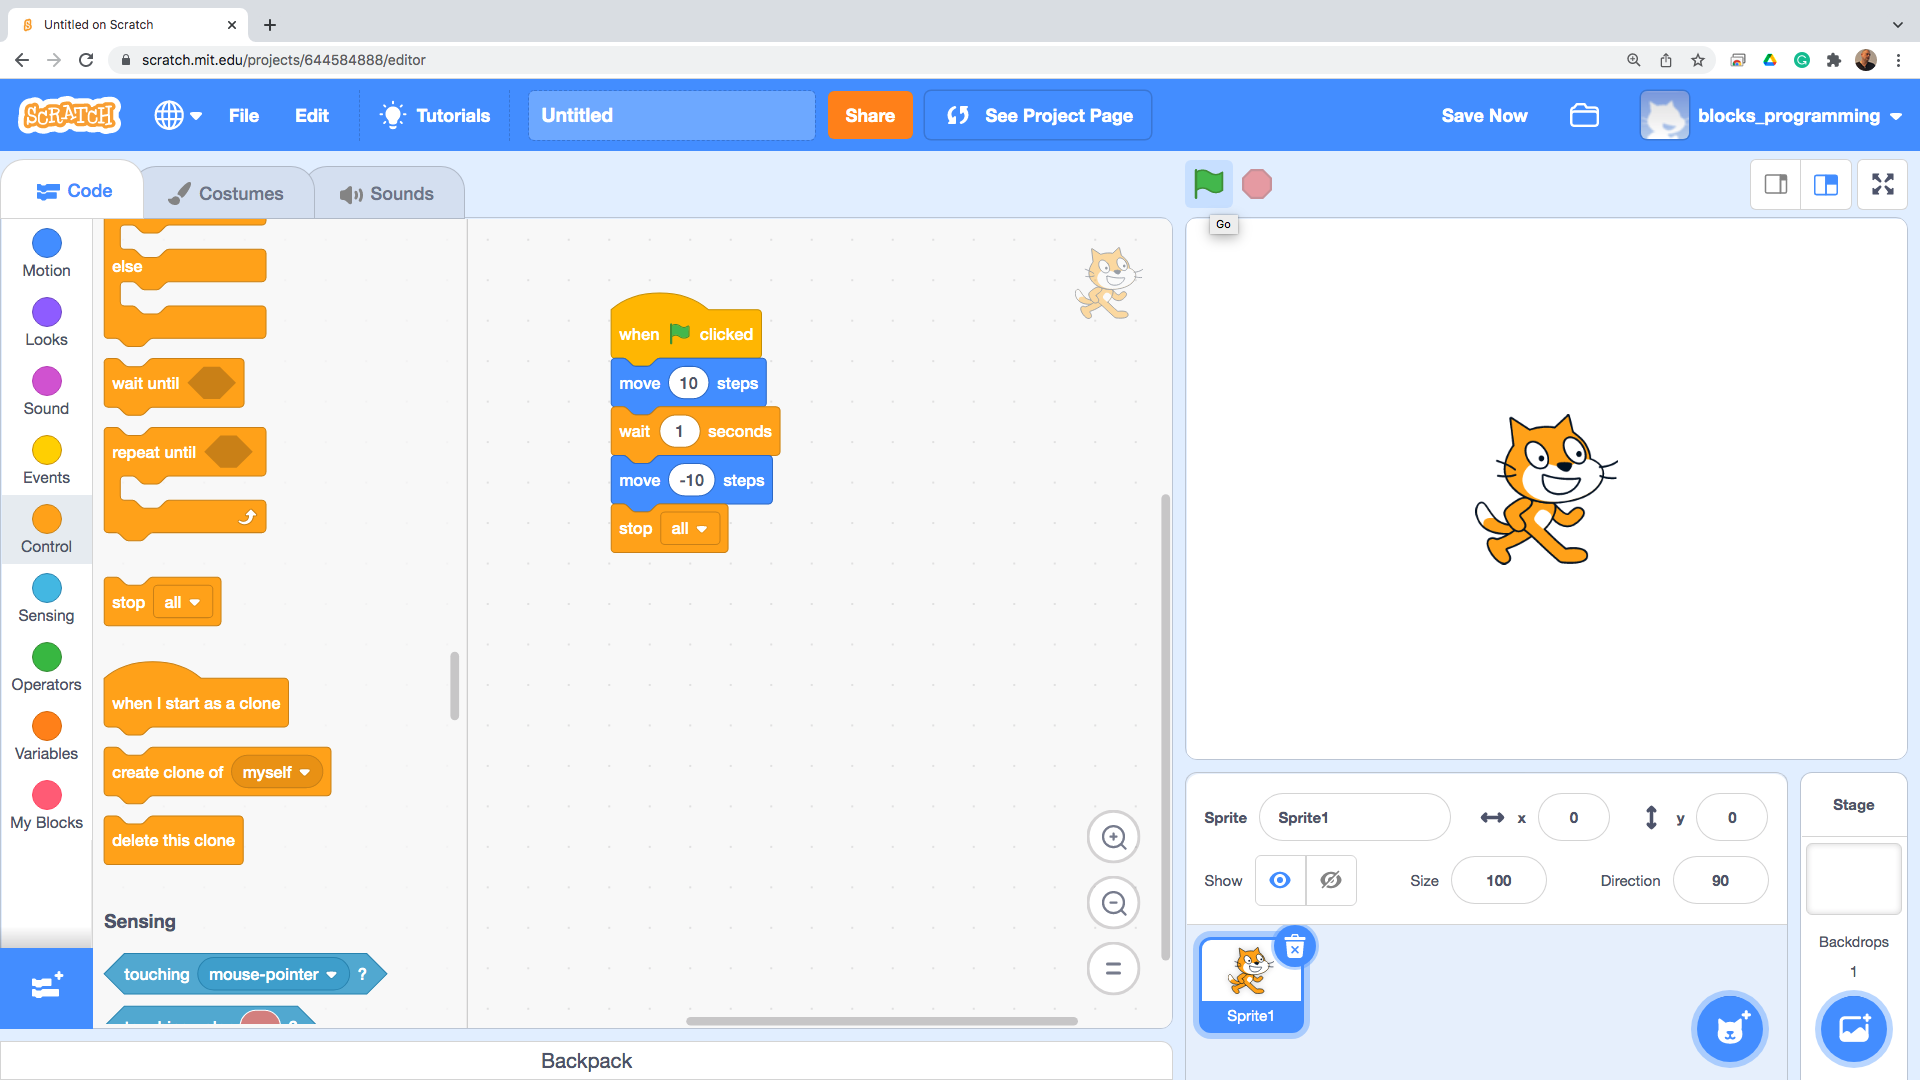
\includegraphics[width=1.0\linewidth,height=0.5\linewidth]{fig0018.png}
  \caption{Изпълнение на програмата}
\label{fig0018}
\end{figure}

Всяка програма, която се пише в Scratch се помества в отделен проект. Достъп до всички проекти на потребителя може да се получи от менюто „My Stuff“, което е част от списъка с опции за боравене с регистрирания потребител (Фиг. \ref{fig0019}).

\begin{figure}[H]
  \centering
  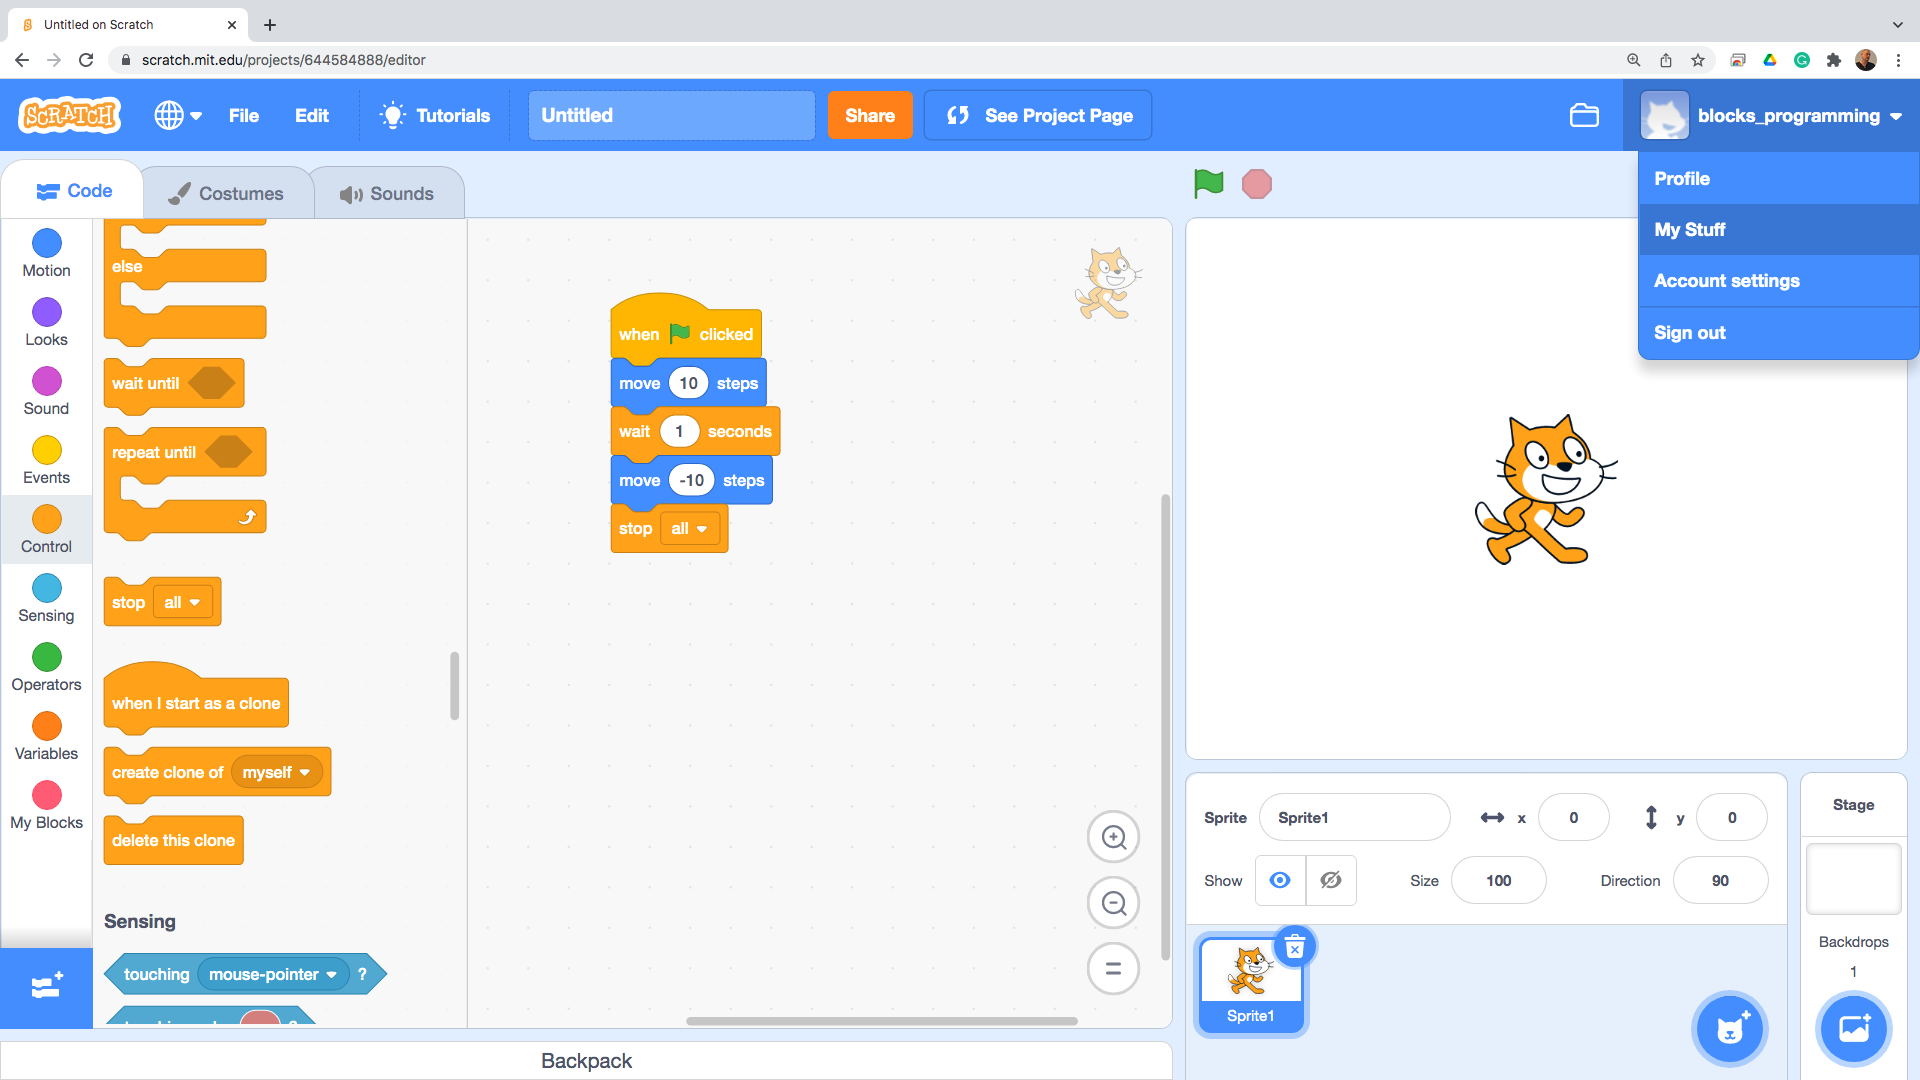
\includegraphics[width=1.0\linewidth,height=0.5\linewidth]{fig0019.png}
  \caption{Меню за организация на проектите}
\label{fig0019}
\end{figure}

Първоначално, всеки проект има служебно име (Фиг. \ref{fig0020}), което в последствие може да бъде променено. Едно от най-атрактивните предимства на програмната среда е, че проектите на потребителите могат да се споделят (Sharing) с много широка аудитория. Това позволява бърз трансфер на знания и умения, както и оценка за положения труд. 

\begin{figure}[H]
  \centering
  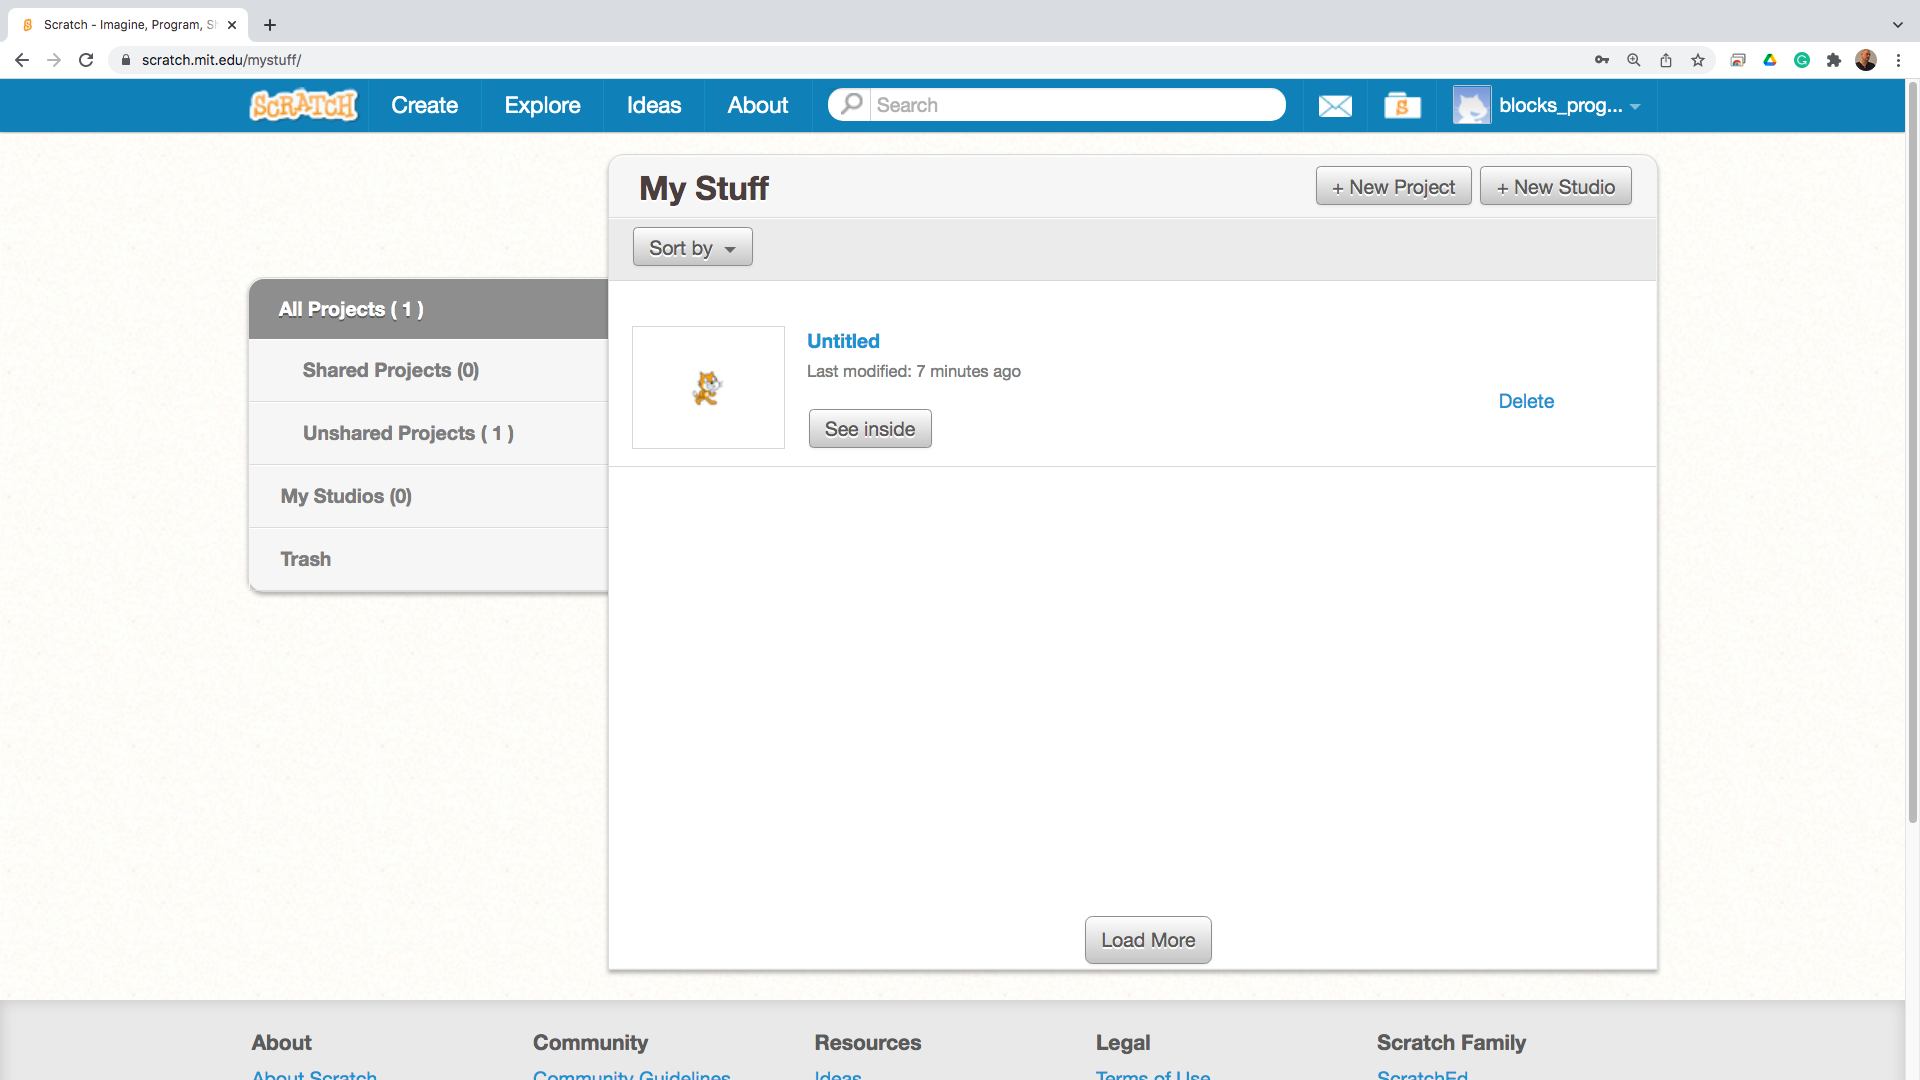
\includegraphics[width=1.0\linewidth,height=0.5\linewidth]{fig0020.png}
  \caption{Списък с проекти}
\label{fig0020}
\end{figure}

Най-голямото очарование блоковите езици получават от факта, че писането на инструкциите и формирането на цялостна програма прилича на подреждането на пъзел. Почти всички деца обичат да редят пазели. Харесват ярките цветове и красивите картини. Когато чарът на класическите пъзели се пренесе в една толкова атрактивна област, каквато е програмирането, резултатите могат да бъдат смайващи. 

\section{Първи стъпки в App Inventor}
